%% josis.tex 1.4   2016-09-15    JoSIS latex template
%------------------------------------------------------------------
% Filename: josis_template.tex
%
% This file is intended as a template for typesetting articles for the
%
%                        Journal of Spatial Information Science.
%
% Please edit this template to generate your own formatted manuscripts
% for submission to JOSIS. See http://josis.org for further details.
%


%%% JOSIS checks in typesetting
%%% * All titles and sections lower case *EXCEPT short title  [ ]
%%% * Remove author postal addresses, only have geographic places and institutions [ ] 
%%% * Consistent use of Section, Figure, Table (capitalized and in full) [ ]
%%% * 10 keywords (and all lower case) [ ]
%%% * Remove all avoidable footnotes [ ]
%%% * Use double quotation marks (``'' not "" or `') [ ]
%%% * Punctuation inside quotations [ ]
%%% * E.g. and i.e. followed by comma [ ]
%%% * cf. followed by tilde [ ]
%%% * Itemize and enumerate correctly punctuated [e.g., "1. x, 2. y, and 3. x." ]
%%% * And/or lists using American English punctuation (e.g., "x, y, and z") [ ] 
%%% * Bibliography (e.g., en-dashes for number ranges, consistent "Proc.~" for Proceedings of..., etc.) []
%%% * Acknowledgment style use section* [ ] 
%%% * et al. no italics, but with dot  [ ] 
%%% * All captions end with full stop  [ ] 
%%% * Table captions under, not over table  [ ]
%%% * Adjust urls with burlalt [ ] 
%%% * Check correct use of hyphens, emdashes, endashes  [ ]
%%% * Perform spell check  [ ] 

%%% JOSIS checks directly before publication 
%%% Check DOI, page numbers on article and web site. [ ]
%%% Update web site with final title, abstract, keywords. [ ] 
%%% Build with distiller for DOI links. [ ]


% Required documentclass definition for JOSIS
\documentclass{josis}
% Use class below for preprint
% \documentclass{josis-preprint}
\usepackage{hyperref}
\usepackage[hyphenbreaks]{breakurl}
\usepackage{booktabs}
\usepackage{stmaryrd}
\usepackage[T1]{fontenc}
\usepackage{cite}

% Suggested packages for algorithm formatting
\usepackage{algorithm}
%\usepackage{algorithmic}
\usepackage{algpseudocode}
\usepackage{comment}

\usepackage[table]{xcolor}
\usepackage{amssymb,amsmath}

\renewcommand{\topfraction}{0.9} 
\renewcommand{\textfraction}{0.1}

% Page setup and overhangs
\sloppy
\widowpenalty=10000
\clubpenalty=10000
\hyphenpenalty=75

% Article details for accepted manuscripts will be added by editorial staff
% Omit year if article in press
% Omit number if article under review

% commented out for preprint:
\josisdetails{%
   number=N, year=YYYY, firstpage=xx, lastpage=yy, 
  doi={10.5311/JOSIS.YYYY.II.NNN},
   received={December 24, 2015}, 
   returned={February 25, 2016},
   revised={July 13, 2016},
   accepted={September 5, 2016}, }

\newcommand{\mydoi}[1]{\href{https://doi.org/#1}{doi:\protect\detokenize{#1}}}

%\renewcommand{\UrlLeft}{http:\sslash}
%\DeclareUrlCommand\myurl{\def\UrlLeft{}\def\UrlRight{}%
%\urlstyle{tt}}

\urlstyle{rm}
\makeatletter
% Inspired by http://anti.teamidiot.de/nei/2009/09/latex_url_slash_spacingkerning/
% but slightly less kern and shorter underscore
\let\UrlSpecialsOld\UrlSpecials
\def\UrlSpecials{\UrlSpecialsOld\do\/{\Url@slash}\do\_{\Url@underscore}}%
\def\Url@slash{\@ifnextchar/{\kern-.11em\mathchar47\kern-.2em}%
    {\kern-.0em\mathchar47\kern-.08em\penalty\UrlBigBreakPenalty}}
\def\Url@underscore{\nfss@text{\leavevmode \kern.06em\vbox{\hrule\@width.3em}}}
\makeatother

\hypersetup{
colorlinks=true,
linkcolor=black,
citecolor=black,
urlcolor=black
} 

% Add the running author and running title information
\runningauthor{\begin{minipage}{.9\textwidth}\centering Granell et al.\end{minipage}}
\runningtitle{Impact of reproducible research practices in GIscience domain}

% Document begins
\begin{document}
%\setcounter{page}{33}


% Insert your own title
\title{Longitudinal assessment of research in GIScience domain shows a positive impact of reproducible research practices}

%Impact of evolving publishing requirements on open and reproducible practices: A longitudinal assessment in the GIScience domain}

%Impact of reproducible paper guidelines on computational papers: A longitudinal study on the AGILE and GIScience conference series}

% Insert your manuscipts authors, affiliations, and addresses
\author[1]{Carlos Granell} % http://orcid.org/0000-0003-1004-9695
\author[2]{Frank O. Ostermann} % https://orcid.org/0000-0002-9317-8291
\author[3]{Daniel Nüst} % https://orcid.org/0000-0002-0024-5046
\author[4,5]{Peter Kedron} % https://orcid.org/0000-0002-1093-3416
\author[6]{Eftychia Koukouraki} % https://orcid.org/0000-0003-0928-1139
\author[1]{Miguel Matey-Sanz} % https://orcid.org/0000-0002-1189-5079
\author[7,8]{Rémy Decoupes} % https://orcid.org/0000-0003-0863-9581
\author[1]{Sergio Trilles} % https://orcid.org/0000-0002-9304-0719
\author[9]{Anita Graser} % https://orcid.org/0000-0001-5361-2885
\author[3]{Tom Niers} % https://orcid.org/0000-0002-5746-8590


\affil[1]{Institute of New Imaging Technologies, Universitat Jaume I, Castellón, Spain}
\affil[2]{Faculty of Geo-Information Science and Earth Observation (ITC), University of Twente, Enschede, The Netherlands}
\affil[3]{Department of Geosciences, Technische Universität Dresden, Dresden, Germany}
\affil[4]{Department of Geography, University of California Santa Barbara, Santa Barbara, United States}
\affil[5]{Center for Spatial Studies and Data Science, University of California Santa Barbara, Santa Barbara, United States}
\affil[6]{Institute for Geoinformatics (ifgi), University of Münster, Münster, Germany}
\affil[7]{TETIS, Univ. Montpellier, AgroParisTech, CIRAD, CNRS, INRAE, Montpellier, France}
\affil[8]{INRAE, Montpellier, France}
\affil[9]{AIT Austrian Institute of Technology, Vienna, Austria}



\maketitle

% Add 5-10 keywords for every submission
\keywords{GIScience, reproducible research, reproducibility, computational science, data science, open science, meta-science, meta-research, science policy, open access}

% Add a short abstract of 150-250 words
\begin{abstract}

Reproducibility is increasingly recognised as a cornerstone of rigorous science, prompting many publishers to require full documentation, data and software access, and archiving of study materials. 
Yet prior work shows that such practices, that are essential for communicating research transparently, remain comparatively low in the Geographic Information Science (GIScience) research community. 
To address this challenge, the AGILE conference series introduced the AGILE Reproducible Paper Guidelines for submissions in 2020. 
This study evaluates the effect of those guidelines and their implementation by a reproducibility committee.
We investigate the evolution of the potential reproducibility of publications from the AGILE and the GIScience conference series, respectively, through a longitudinal analysis of full papers published before and after the introduction of the guidelines and corresponding review procedures.
We assessed every full paper from both venues published between 2016 and 2024 using a rubric that classifies the availability of data, computational methods, and results. Results indicate that the AGILE Guidelines and reproducibility reviews measurably improved the potential reproducibility of AGILE publications. The comparison with GIScience papers further suggests that clear, enforced guidance is a meaningful lever for change. Our findings demonstrate the value of institutional/community policies for fostering reproducible research in GIScience and identify pathways for further improvement.
\end{abstract}

% Your main text begins here. 
\section{Introduction}
\label{sec:intro}

\subsection{Motivation}
\label{sec:motivation}
Computational research relies on the ability to verify, build upon, and critically evaluate published findings. 
However, across disciplines, researchers have documented persistent challenges when attempting to reproduce computational results~\cite{barba_terminologies_2018, nasem_reproducibility_2019, DiCosmo2025} from published papers, even when authors provide code and data~\cite{konkol_computational_2019, obels_analysis_2020, kambouris_computationally_2024, brodeur_mass_2024}. 
In geographic information science~(GIScience), a small but growing literature suggests this reproducibility gap may be particularly acute~\cite{konkol_computational_2019, koukouraki_map_2023}. 
GIScience research often depends on specific software versions, computational environments, proprietary datasets, and undocumented analytical decisions that are difficult to reconstruct from published descriptions alone.
To address these challenges, leading GIScience journals and conferences have adopted data and code sharing policies that establish standards for code availability, data sharing, and computational documentation.
The extent to which such guidelines improve the reproducibility of published computational research is an actively researched question \cite{stodden_empirical_2018, Hardwicke2018, Fiar2024}.

We have laid the conceptual and technical groundwork to address this question in a pair of studies that examine publications from the Association of Geographic Information Laboratories in Europe (AGILE) and the GIScience conference series \cite{nust2018, ostermann2021}. 
In these studies, we evaluated the potential reproducibility of the conference publications based on the availability of the materials involved, discussed the state of reproducibility in comparison to other disciplines, and suggested actions to improve reproducibility within the GIScience community. We specified and used an \emph{assessment rubric} to evaluate the potential reproducibility, following a similar approach across studies~\cite{nust2018, ostermann2021}. In this rubric, we categorise the availability of input data, methods, and results into four levels of (non-)availability, transparency, and openness: (U) unavailable, (D) documented, (A) available, and (O) available, open, and permanent.
These levels document to what degree the necessary conditions for a reproduction were present according to the rubric, but neither study attempted to actually reproduce any of the papers analysed.
The second study on the GIScience conference series~\cite{ostermann2021} essentially acted as a replication of our first study on the AGILE conference series~\cite{nust2018}, using the same methodology on a different pool of input data.

Our analyses revealed that ``reproducibility and replicability have not been a core concern in the contributions''~\cite[pp 2:2]{ostermann2021} in either conference series \cite{nust2018, ostermann2021}, which led us to make a series of recommendations for process improvements.
These recommendations identified improvements to author guidelines and peer review procedures as important levers capable of improving reproducibility practices around computational workflows~\cite{DiCosmo2025}.
A key outcome of our study \cite{nust2018} was the development and publication of the AGILE Reproducible Paper Guidelines (hereafter referred to as \textit{the AGILE Guidelines}) in 2019.
These AGILE Guidelines were revised in late 2020~\cite{nust2020_guidelines} and have been gradually implemented at the AGILE conference series, along with the establishing of a Reproducibility Committee responsible for performing reproducibility reviews of all accepted full papers.
No similar set of reproducibility guidelines or review process was adopted by the GIScience conferences series, creating an opportunity to evaluate the impact of the AGILE guidelines by assessing differences in reproducibility levels across conferences. 

In this work, we build on these foundations and investigate the impact of the AGILE Guidelines on the potential reproducibility of AGILE conference papers to determine if there is measurable change across conference editions.
Using an updated compatible rubric that remains comparable to our earlier studies, we compare the changes in the potential reproducibility of papers published by the AGILE conference over time and to those of papers published by the GIScience conference.
These comparisons allow us to assess the impact of the AGILE Guidelines, and establish whether using them as part of code checking procedures during the conference peer-review process contributes to making conference publications more reproducible.

The remainder of the article is structured as follows: The next sections present the research questions and provide an overview of related work, followed by a detailed description of the methods, before the results are presented in Section~\ref{sec:results}. The article concludes with an in-depth discussion and interpretation on methods and findings, before outlining future research directions.

\subsection{Research questions and expectations}
\label{sec:methods:questions}

%This study uses a slightly but compatibly adjusted assessment rubric to investigate whether the introduction of the Guidelines has led to significant improvements in the level of reproducibility of the papers published in the AGILE conference proceedings. 
%The papers from the GIScience conferences, where no similar policy shift toward reproducibility has yet occurred, serve as a baseline.

\noindent \textbf{Question 1 (AGILE-only scope)}: Has the level of potential reproducibility of AGILE papers increased after the introduction of the AGILE Guidelines and reproducibility reviews?

\noindent \textbf{Question 2 (GIScience-only scope)}: Has the level of potential reproducibility changed for the GIScience conference series during the same period?

\noindent \textbf{Question 3 (AGILE-GIScience scope)}: Is there an observable difference in the change in potential reproducibility for papers published by the AGILE and GIScience conferences during this period?

% Prereg study
%\textbf{Question 3 (AGILE-only scope)}: Do papers required to follow the Guidelines retain the level of reproducibility over time? Specifically, are links and references in papers reaching at least level 2 in the years since the Guidelines were introduced still functional today, and is there a difference in success between reaching level 2 and 3? 

We expect the average level of potential reproducibility in papers published as part of the AGILE conference after the introduction of the AGILE Guidelines and the corresponding reproducibility committee to be higher than the potential reproducibility of papers published before their introduction (Question 1). Furthermore, one might anticipate a steadily increasing trend of the average potential reproducibility level of post-guidelines AGILE papers (2021-2024), as authors may have progressively adapted the AGILE Guidelines to their contributions to the conference. This trend may even exhibit a notable shift corresponding to when the reproducibility reviews began or when the AGILE Guidelines became mandatory. %We expect that post-guidelines AGILE papers will retain the level of reproducibility over time better than pre-guidelines papers. We expect that papers with level 2 in a category will not be able to retain that level over time, yet we are unsure if the additional steps that must be taken to reach level 3 are having an impact, i.e., if level 3 is more sustainable. 
We also expect that, for the GIScience conference, the average level of potential reproducibility in papers will increase due to a general trend in the discipline, but the change will be less than for AGILE (Question 2). 
While any changes in potential reproducibility could be attributed to the AGILE Guidelines (Question 1), Question 3 seeks to discover whether these changes could be a mere coincidence or reflect a general trend in the discipline of GIScience.

\subsection{Related work}
\label{sec:related}

Since the 2020 AGILE conference, the AGILE Reproducible Paper Guidelines~\cite{nust2020_guidelines} have been recommended for all authors and reviewers\footnote{\url{https://web.archive.org/web/20200926160015/https://agile-online.org/conference-2020/call-for-papers-2020}}
% "Submissions are encouraged but not obliged to follow to the AGILE Reproducible Paper Guidelines: https://doi.org/10.17605/OSF.IO/CB7Z8."
and a reproducibility committee has conducted reproductions of accepted full paper submissions~\cite{nust2020improving}. 
The AGILE Guidelines offer extensive advice on open science practices aimed at improving workflow reproducibility of conference papers. 
Importantly, they introduced a mandatory requirement\footnote{\url{https://web.archive.org/web/20210812211908/https://agile-online.org/index.php/conference-2021/call-for-papers-2021}}
% " All submissions have to follow to the AGILE Reproducible Paper Guidelines: https://doi.org/10.17605/OSF.IO/CB7Z8."
that all papers submitted to AGILE conferences after 2020 must include a dedicated section titled \textit{Data and Software Availability} (DASA), where authors disclose and reference the data and software used and/or developed in their reported research, or transparently document a lack thereof or reasons for closedness. 
In addition to describing the obligations of authors, the AGILE Guidelines set out the roles and responsibilities of reproducibility and scientific reviewers,
raising awareness of reproducibility practices and improving the consistency and efficiency of the review process. In other words, the AGILE Guidelines are an integral part of the peer-review mechanism, as the review committees take them into rigorous consideration.

The reproducibility review used to evaluate AGILE conference papers follows the AGILE Guidelines, but does not critically evaluate an entire paper in the manner of traditional peer review. 
Rather, reproducibility reviewers attempt to reproduce a paper's computational workflow and assess in detail the underlying data and computational methods. 
The review process is open and collaborative. 
Authors are given the opportunity to revise their manuscripts and their associated research resources in response to reviewer feedback prior to publication.

In scope and extent, the AGILE reproducibility review is a concrete implementation of the CODECHECK principles~\cite{nust_codecheck_2021}.
These principles enable publication venues (journals, conferences, etc.) to evaluate computer programs underlying scientific papers.
The independent execution of full or partial workflows is carried out by codecheckers, a specialised reviewer role that gives recognition to other  less common profiles in the peer review process, such as early-career researchers, data/software experts (e.g., data stewards, research software engineers) and Open Science enthusiasts. A reproduction grants a timestamped and published CODECHECK certificate (see~CODECHECK~Register~\cite{nust_codecheckersregister_2025}), which in AGILE is called ``Reproducibility Review''\footnote{Access to all AGILE-related certificates at \url{https://codecheck.org.uk/register/venues/conferences/agilegis/}}.
Documenting the workflow execution and the associated conversation between authors and codecheckers benefits all parties involved and increases the availability and transparency of elements crucial to open and reproducible research, as well as for educational purposes.
%CODECHECK certificates are listed in the CODECHECK Register~\cite{nust_codecheckersregister_2025}.

More broadly, the AGILE Guidelines and associated review process exist within an expanding literature on the reproduction and replication of geographic research. 
Work has proceeded along several lines of inquiry. 
Conceptually, geographers have begun to investigate the epistemological role of reproduction and replication within the discipline~\cite{goodchild2021,kedron_geoganaly_2021, kedron_reproducibility_2021} and examine how work in these areas is related to disciplinary research questions~\cite{Wainwright2021, Sui2021, Brunsdon2021, kedron2022}. 
This conceptual work has emphasised that replicability across space and time must be weak due to the ubiquity of spatial heterogeneity, and stressed how variation in the design of reproduction and replication attempts tests different forms of study validity~\cite{kedron2024, kedron2025}. 
Empirically, researchers have attempted to identify the causes of the irreproducibility of geographic analyses~\cite{kedron2024_insights, kedron2025} while also attempting to reproduce and replicate selected studies~\cite{kedron2022_dimaggio, Li2024_geoAI}. 
In addition to the stream of research leading to this study~\cite{nust2018, ostermann2021}, geographers have attempted to replicate analyses of the spatial distribution of COVID-19\cite{paez2022, kedron2024}, reproduce published maps~\cite{koukouraki_map_2023, Koukouraki2024}, and create ``replicability maps'' in GeoAI based research~\cite{Li2024_geoAI}. 
Multi-analyist replication studies~\cite{Aczel2021} are likewise beginning to appear in the literature, signalling the emergence of a new empirical approach to the challenge of replication in geography~\cite{breznau2025}. 

These works have revealed significant reproducibility challenges and prompted broader calls for substantial institutional changes within the GIScience community~\cite{kedron_reproducibility_2021}, in line with the broader scientific landscape~\cite{munafo_manifesto_2017, davis-stober2025}. 
In response to these challenges, recommendations such as introducing reporting checklists or guidelines and adopting reward badges~\cite{dudda_open_2025} have been proposed, and these specific interventions have been implemented at the AGILE conference.
While investigations suggest such interventions have positive effects across disciplines~\cite{stodden_empirical_2018, hardwicke_empirical_2020, dudda_open_2025, breznau2025, Fiar2024}, to our knowledge, no longitudinal study has yet systematically investigated the effects of these policy-related changes in the domain of GIScience. This research addresses this gap by evaluating whether these reforms represent tangible progress toward more reproducible research within the GIScience community.

The analyses presented in this paper closely align with this earlier empirical work but also represent an advancement within the field. 
Whereas previous work has focused on the reproducibility of single studies or paper collections, our work evaluates how potential reproducibility changes within a particular publication venue after the introduction of a specific policy and review process.
This distinction is important because numerous geography journals (e.g. \cite{Cannon2022}) have already introduced similar data and code sharing policies and incorporated some level of materials review into their peer review process. 
If such policies are ineffective, they would represent a significant waste of author and reviewer efforts.


\section{Methods}
\label{sec:methods}

\subsection{Preregistration and overall approach}

To improve the open science practices of this work, we published our intended hypotheses, research objectives, data collection and assessment process, and analysis plans as a preregistration~\cite{nust2023_prereg}.
We further share all data and code--see Section~\ref{sec:dasa}.
In case we deviate from the preregistered research design, we explicitly mention and justify these deviations.

This study improves on prior studies on the assessment of reproducibility~\cite{nust2018,ostermann2021} in a number of ways.
First, it adds a crucial amount of input data to the comparison.
The original studies were focusing on the level of reproducibility of the respective conference's papers, analysing the factors contributing to the observed low levels, and on raising awareness of this problem within the GIScience research community.
These studies could not examine an impact of the AGILE Guidelines or workflow evaluation because they preceded their introduction at AGILE conference.
Second, the prior studies looked at conferences separately while this work uses robust non-parametric statistics to quantify and compare the assessment of the two conference series based on three hypotheses.
Third, we employ a newly formalised reproducibility assessment protocol (see Section~\ref{sec:methods:assessment}) based on the assessments of previous studies, thereby increasing chances for successful replication of the protocol.
The protocol allows us to combine experienced contributors with a new group of assessors yet stringently ensure consistency and quality of the assessment.

\subsection{Data collection process and corpus}
\label{sec:methods:corpus}

The AGILE and GIScience conference series follow two different rhythms. The AGILE conference is held annually, while the GIScience conference is a bi-annual event.
Further, the COVID pandemic led to cancelled conference editions in 2020 within the observed time frame and changed publication patterns for the GIScience conference series.

The publication of the AGILE Guidelines, the \emph{intervention}, took place in 2020. The DASA section remained optional for authors submitting to the conference in that year. 
Therefore, we consider proceedings published before 2019 and during that year are part of the \emph{pre-intervention} period, published in 2020 are part of the \emph{transitional} period, and published in 2021 and later are part of the \emph{post-intervention} period.
All papers from the transitional period were excluded from the analyses in Sections~\ref{sec:results:assessment}~and~\ref{sec:results:hypothesis}.

The preparation and analysis for this study began in 2023. 
For a sufficiently large and balanced paper corpus, we decided to match the post-intervention proceedings and papers from both conferences with a similar number of pre-intervention proceedings and papers. 
This means that the three post-intervention proceedings from AGILE and the two post-intervention proceedings from GIScience were matched with an equal number of pre-intervention editions, resulting in coverage of a 9-year period (details see below). 
We consider n>15 papers/year to be adequate to allow for statistical inference and testing. No sampling was done within a year; instead, all papers from a year were assessed.   
While one could argue that more data is always preferable, we also had to keep feasibility in mind. 
Further, looking back too far in time would bias the analysis towards a positive result, since a decade ago, reproducibility was not at all on the GIScience agenda.

For this study, we initially considered in the preregistration all published full papers in the AGILE proceedings of the 2017, 2018, 2019, 2021, 2022, and 2023 conference editions. 
Because the AGILE 2024 proceedings became available before the assessment, we decided to include them in the paper corpus. 
For the GIScience conference, the GIScience 2021 proceedings included two volumes: papers submitted and published in 2020 (GIScience 2021 Part I) and the papers submitted and published in 2021 (GIScience 2021 Part II). Therefore, we excluded the GIScience 2021 Part I proceedings from the analysis as a transitional year, like we did with the AGILE 2020 papers. Thus, all published full papers of the 2016, 2018, 2021 (Part II), and 2023 GIScience conferences were included.

Full texts of the conference papers were accessed directly from the publishers' websites (Springer, LIPICS, Copernicus) for assessment. Access to copyrighted content, particularly those from Springer (GIScience 2016, AGILE 2017, AGILE 2018, and AGILE 2019), required institutional access granted to some authors' universities.
These conference papers were downloaded locally to facilitate their assessment but were not publicly disclosed during the study.
In total, 224 full articles were collected, 78 from GIScience and 146 from AGILE, as listed in Table~\ref{tab:corpus}.
While all were assessed, articles published in the transition year (2020) for both conferences were excluded from some analyses, so the number of articles included before and after the intervention was 186 in total, 62 from GIScience and 124 from AGILE.

\begin{table}
\centering
\begin{tabular}{lrcrr}
\hline
Year & Conference & Number papers & Publisher & Open Access \\
\hline
2016 & GIScience 2016 &  21 & Springer & N  \\
2018 & GIScience  2018 &  17 & LIPICS & Y  \\ 
2020 (transition) & GIScience  2021 Part I &  16 & LIPICS & Y \\ 
2021 & GIScience  2021 Part II &  13 & LIPICS & Y  \\ 
2023 & GIScience  2023 &  11 & LIPICS & Y  \\ 
 & \textbf{Total} & \textbf{78}  &   \\
 & \textbf{Total w/o transition year} & \textbf{62} &    \\

\hline

2017 & AGILE 2017 & 20 & Springer & N \\ 
2018 & AGILE 2018 & 19 & Springer & N  \\
2019 & AGILE 2019 & 19 & Springer & N  \\
2020 (transition) & AGILE 2020 & 22 & Copernicus & Y  \\
2021 & AGILE 2021 & 16 & Copernicus & Y  \\
2022 & AGILE 2022 & 22 & Copernicus & Y  \\
2023 & AGILE 2023 & 14 & Copernicus & Y  \\
2024 & AGILE 2024 & 14 & Copernicus & Y  \\
 & \textbf{Total} &  \textbf{146} &   \\
 & \textbf{Total w/o transition year}  & \textbf{124} &  \\
\hline
\end{tabular}
\caption{Paper corpus. Source: \texttt{02\_methods.qmd}~\cite{data}.}
\label{tab:corpus}
\end{table}

A summary of the collected data elements is available at \cite{data}, which includes the dataset and code used to create all tables and figures in this study, as well as related documentation, such as a data sheet to describe each column in the dataset~\footnote{\url{https://github.com/nuest/reproducible-research-giscience-longitudinal-study/tree/main/data-clean}}. This dataset contains basic bibliographic metadata of eligible articles and scores from the reproducibility assessment process.

\subsection{Assessing potential reproducibility}
\label{sec:methods:assessment}

We recruited assessors by email to complete the assessment of papers (October 2024). Assessors were selected based on previous published work on reproducibility and/or former members of the Reproducibility Committee of the AGILE conference series. In total, eight assessors joined the study to evaluate the selected articles and co-author the final study.

\subsubsection{Assessment protocol}
\label{sec:methods:assessment:protocol}

Continuing prior work, our goal was to assess the level of potential reproducibility of a given article without performing an actual computational reproduction. To effectively better integrate new assessors and document implicit knowledge from previous studies~\cite{nust2018, ostermann2021}, we compiled the Assessment Protocol~\cite{assessment_protocol}, which documents a set of practical rules and recommendations for the reproducibility assessment process and discussions about divergent assessments.
It includes instructions for determining whether an article is considered conceptual. Literature studies, review papers, or opinions are out-of-scope for this study, unless they include even a small case study or descriptive statistics, for example.
% Text from the assessment protocol:
% First, read the abstract and possibly the introduction fully to get an idea of what the paper is about. If it does not use any computational analysis, then it's out-of-scope for this study and you may make this decision based on the abstract and introduction.
% Examples of such out-of-scope papers are: purely conceptual papers, literature studies, review/state-of-the-art papers, or proposed methodologies, guidelines, or opinions/reflections. However, even a small case study to support the main (conceptual) argument or descriptive statistics about literature turn this into a paper within scope!
The protocol also includes a rubric and examples to help assessors rate the potential reproducibility level of a non-conceptual article. This rubric has been revised to improve clarity and consistency based on experiences from previous assessments, while maintaining comparability of the main observed properties.

Figure~\ref{fig:rubric} illustrates the four criteria of the rubric. The \textit{Input data} and \textit{Results} criteria remain unchanged with respect to initial version of the rubric~\cite{nust2018, ostermann2021}. The former ``Methods'' criterion, which included categories for preprocessing, analysis, and computational environment in previous studies, has been simplified into a single criterion: \textit{Methods, analysis, processing}. This change avoids ambiguity and disagreements over assigning methodological steps to either preprocessing or analysis. Furthermore, the distinction did not add analytical value to the assessment of reproducibility and the broader category still captures the full range of relevant procedures. Additionally, the \textit{Computational environment} is now treated as a separate, fourth criterion. This reflects its broader role in computational research and data science, encompassing all code and infrastructure used for both analysis and result presentation. Finally, numeric levels previously used in the rubric have been replaced with descriptive labels and single-letter codes. This enhances interpretability, because the levels were always only ordinal, and avoids any misinterpretation as to the differences in value between the labels, because efforts of going from one level to the next and the impact of a higher level compared to a lower one are far from equal steps or linear relationships.
The data preparation steps~\cite{data} includes renaming of the variables for consistency of the output data with this manuscript.
The UDAO levels are, in ascending order of potential reproducibility: undocumented (U); documented (D), documented and available (A); documented, available, and open (O); and ``NA'' retained for not applicable. 
For the \textit{Computational environment} criterion, only a binary evaluation (True/False) is applied, recognising the challenges from past assessments to consistently assigning more granular levels.

\begin{figure}[tbh]
\centering
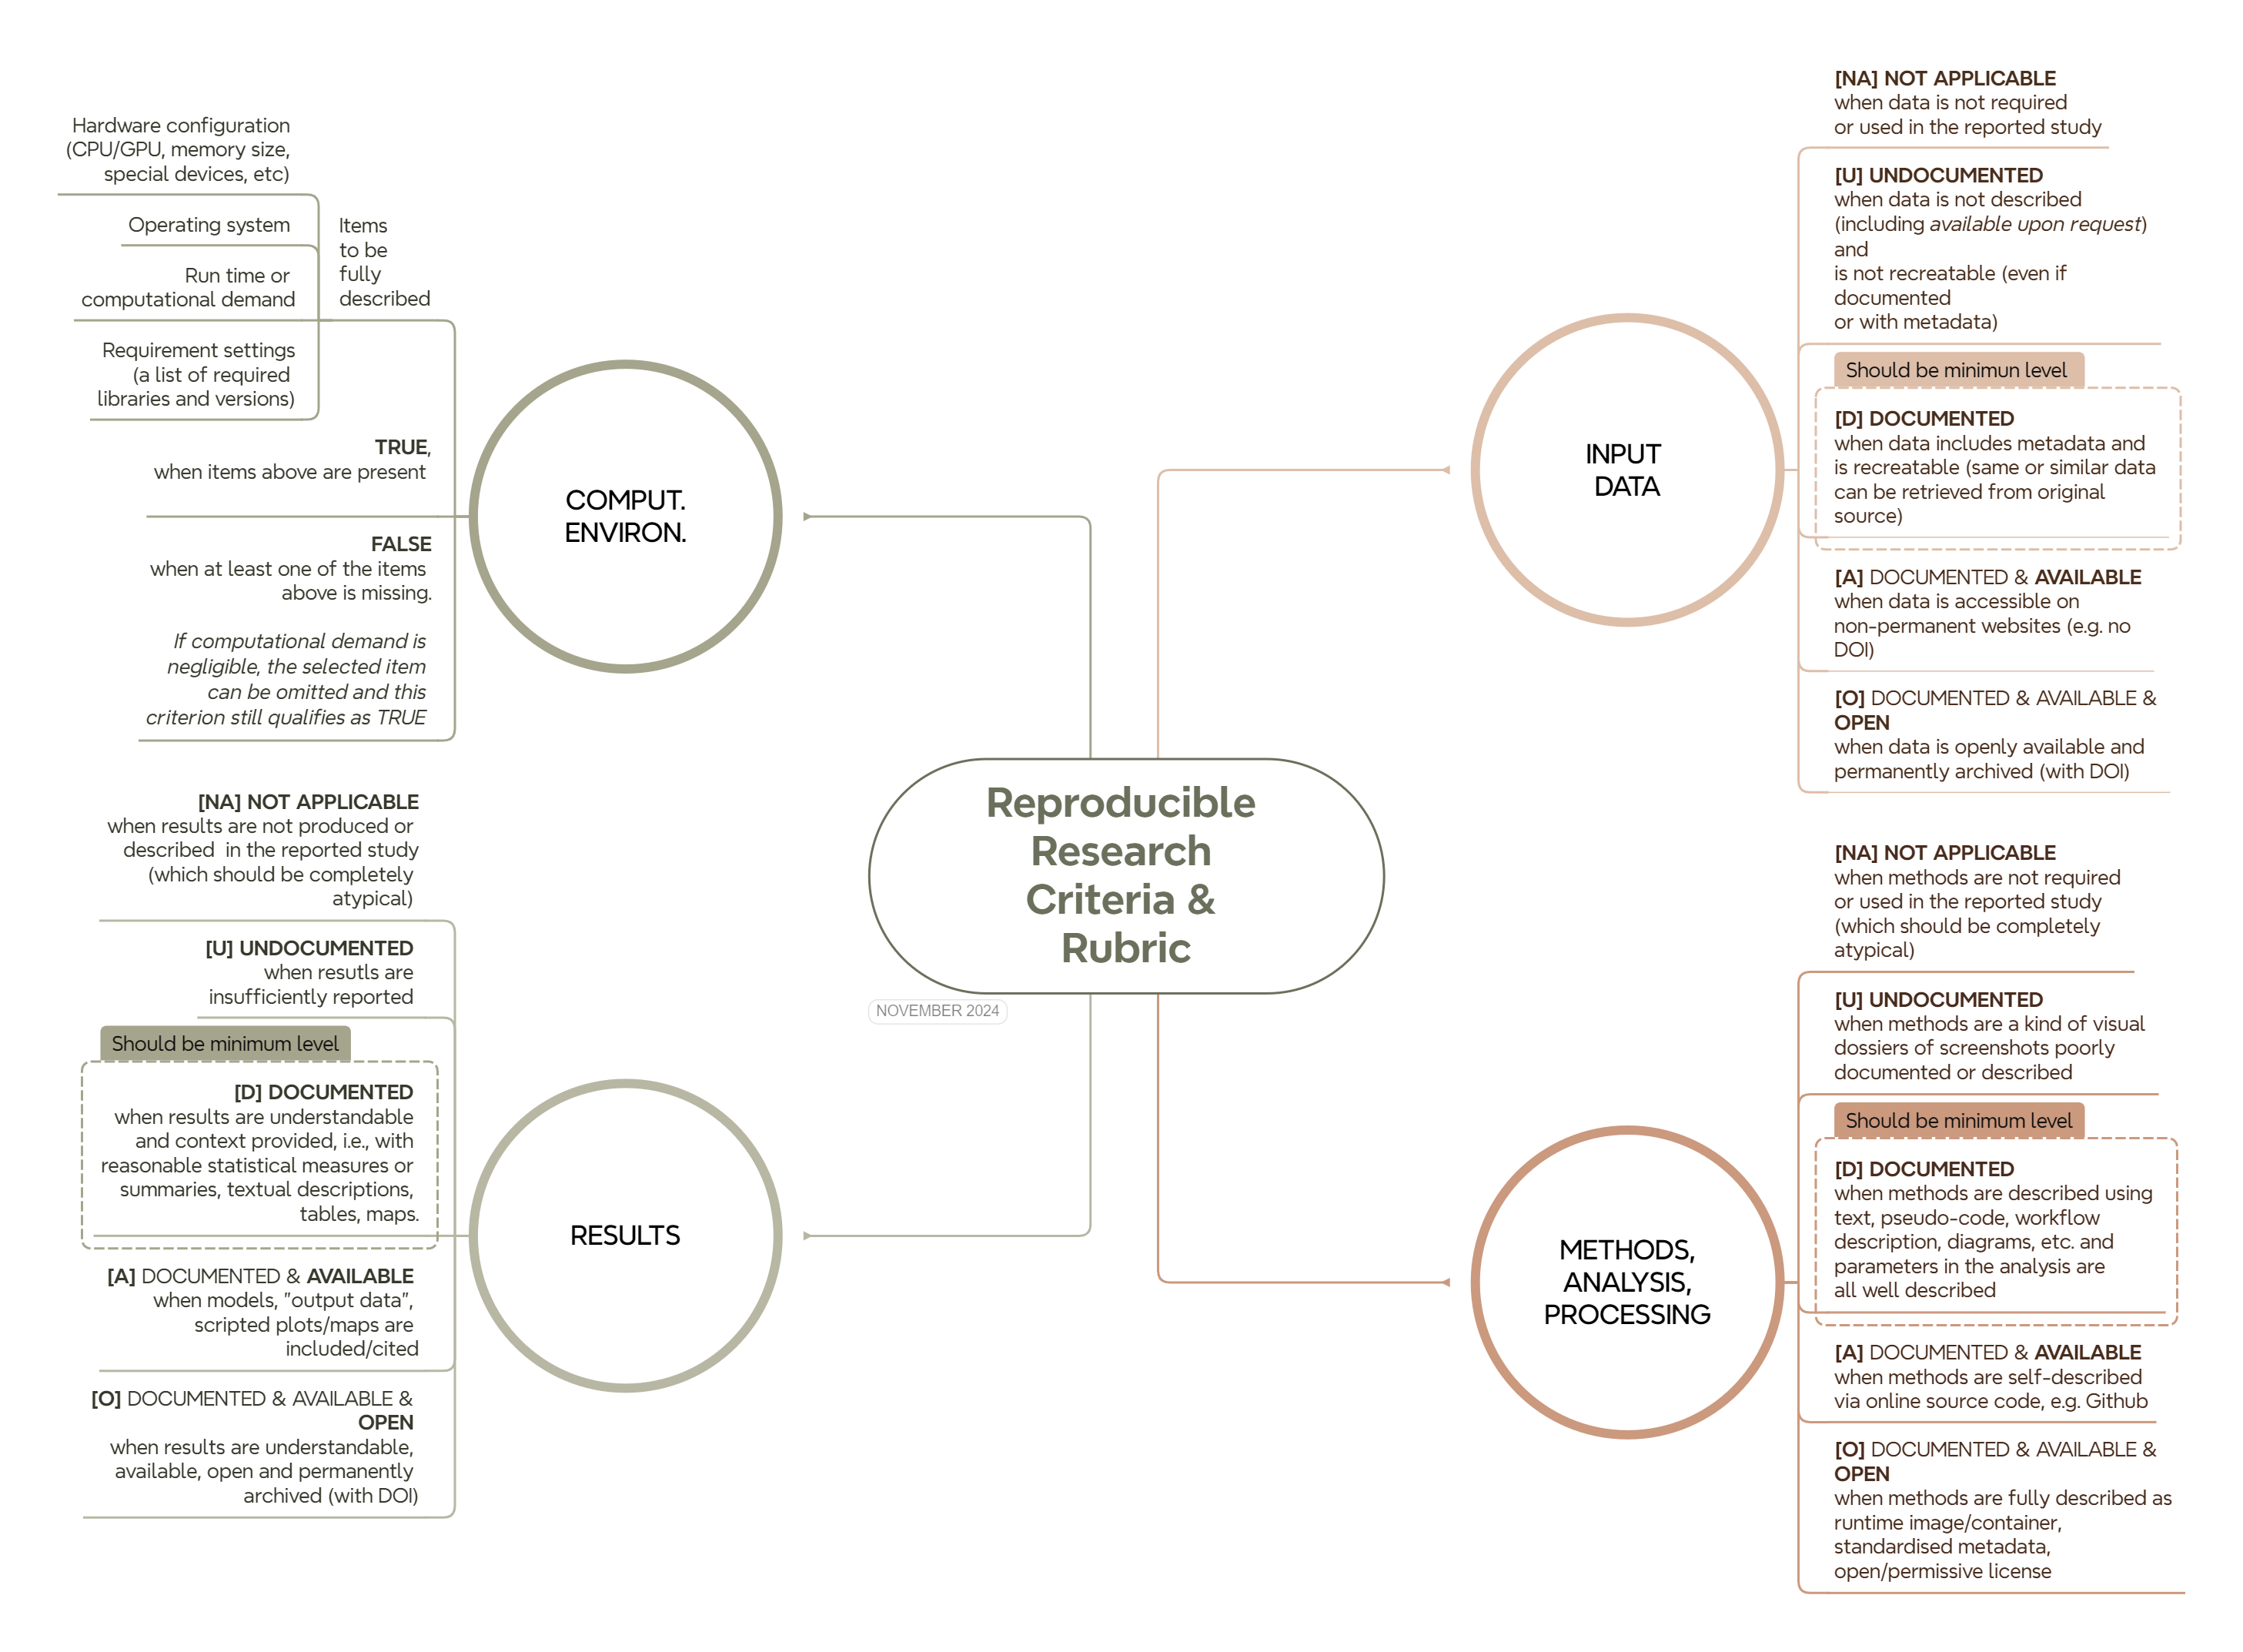
\includegraphics[width=\textwidth]{img/Assessment Rubric v6.png}
\caption{Criteria and rubric for assessing potential reproducibility of a paper~\cite{assessment_protocol}.}\label{fig:rubric}
\end{figure}


\subsubsection{Assessment implementation}
\label{sec:methods:assessment:process}

Each conference paper was independently assessed by two assessors, the first of whom (henceforth A1) had prior experience in evaluating potential reproducibility using the original protocol~\cite{nust2018, ostermann2021}.
% anonimised: Carlos Granell or Frank Ostermann, both of whom
% anonimised: and have been involved in the AGILE Conference Reproducibility Committee since the beginning
The second assessor (A2) was a pool of nine researchers who had varying levels of experience in assessing potential reproducibility. Through this pairing, we aimed to ensure a balanced level of assessment expertise for each paper. All assessors had access to the Assessment Protocol~\cite{assessment_protocol}, see Section~\ref{sec:methods:assessment:protocol}, as a guiding document to qualitatively evaluate each paper. It should be noted, that each assessor was encouraged to record relevant observations, sources (e.g., whether important pieces of information were found in supplementary information), and decisions (e.g., interpretations of phrases or decisions made in borderline cases) during the assessment process.

The first step was for each of the two A1s to select entire years of conference papers to assess. Assessments were completed between May and July 2024 and documented in a shared online spreadsheet. The assignment strategy deviated from the original preregistration study in which ``each assessor of a paper had to be randomly assigned''. This deviation was made to expedite the assessment process and did not affect significantly the initial methodology proposed in the preregistration.

The second step implemented a continuous, batch-based assessment strategy (see Table~\ref{tab:batches}) for the A2s: We divided the total number of papers into four batches, based on the order identified in the preregistration~\cite{nust2023_prereg} (``The assessment begins with the years closest to the intervention [...] and then alternatively expands to earlier and later years [...]``). Each A2 was randomly assigned between 25 and 27 papers in total, distributed equally among the four batches. They were instructed to complete their assignments in batches, that is, complete all paper assessments in batch 1 before moving on to batch 2. In case of a conflict of interest, an A2 assessor could exchange a paper with another assessor. All A2s recorded their assessment in a spreadsheet without knowing any assessments from A1s. The second step of the assessment was completed between November 2024 and February 2025.

\begin{table}
\centering
\begin{tabular}{crc}
\hline
Batch & Conferences & Number of papers\\
\hline
1 & AGILE 2019, AGILE 2021, GIScience 2021 (Part I and II) &  64 \\
2 & AGILE 2018, AGILE 2022, and GIScience 2018 &  58 \\ 
3 & AGILE 2017, AGILE 2023, and GIScience 2023 &  45 \\ 
4 & AGILE 2020, AGILE 2024, and GIScience 2016 &  57 \\ 
\hline
\end{tabular}
\caption{Conference series grouped into batches for A2's assessment. Source: \texttt{02\_methods.qmd}~\cite{data}.}
\label{tab:batches}
\end{table}

Once the assessment process was completed, we proceeded to consolidate the separate evaluation spreadsheets into one file to examine and resolve disagreements and inconsistencies for each paper, as described next. 

\subsubsection{Resolving assessor disagreements}
\label{sec:methods:assessment:disagreement}

%The results of the assessments are presented to fellow assessors, including relevant comments, to overall align the individual perspectives. In case of disagreement between assessors, arguments for and against a certain reproducibility level will be discussed amongst a group of assessors until a consensus is reached. Inter-rater agreement will be recorded and evaluated separately. Two independent assessors per paper increase the objectivity of the final assessment. The discussion of disagreements and conducting the assessment one year at a time is helpful in aligning the interpretation of criteria and, in rare cases, may lead to an adjustment of similar cases in other papers. The assessment begins with the years closest to the intervention (2020 for AGILE, 2021 for GIScience) and then alternatingly expands to earlier and later years (2019, 2021, 2022, 2018, 2023, 2016).

Based on the joint dataset with the independent evaluations from A1 and A2, A1s analysed each paper's assessment quantitatively and qualitatively as follows to resolve inconsistencies. 

% STEP 1 Interrater and coding categoriesof causes of disagreement.
% **no disagreement**: Reviewers' scores are the same in all dimensions (conceptual paper, data, methods, results)
% **borderline conceptual paper**: Disagreement are due to a different understanding whether a paper is completely conceptual; some reviewers may see a paper that only has demonstrative, synthetic example data as not “data-based” or empirical and exclude it from the assessment.
% **annotation inconsistencies**: Disagreements are due to errors in the level/score selected given the written notes of either reviewer. No matter the dimension where inconsistencies are.
% **uncertain assessment (according to protocol assessment)**: either reviewer wrote that they are unsure about level x or y, so we could just change that to the level matching the other reviewer.
%**significant disagreement**: when reviewers' notes (or lack of notes) cannot explain differences in assessment and conversation to get an agreement is necessary and/or checking again the paper is required.
First, we looked at general trends in interrater (dis)agreement.
%Whether assessors agreed on conceptual papers or not was, from an analysis point of view, a similar question/concern to whether they agreed on any of the other assessment dimensions. 
We checked disagreements for conceptual papers and for the other three criteria, and investigated the sources of disagreement between A1 and A2 by analysing their comments of each paper to record misunderstandings and obvious mistakes in the assessment. Although it was not anticipated at the time of preregistration, we came up with five coding categories that might be potential causes of discrepancies between the individual assessors' scores:

\begin{itemize}
    \item \textbf{No disagreement}: Assessors assigned identical scores across three criteria (\textit{Input data}, \textit{Methods, analysis, processing} and \textit{Results}).

    \item \textbf{Borderline conceptual paper}: Disagreements stemmed from differing interpretations of whether a paper should be classified as conceptual. For instance, some assessors did not consider papers using only synthetic or demonstrative example data as empirical, and thus assigned them as conceptual.

    \item \textbf{Annotation inconsistencies}: Discrepancies resulted from apparent errors or inconsistencies in the selected scores relative to the assessors’ written notes. This type of disagreement applies regardless of which assessment criterion was affected.

    \item \textbf{Uncertain assessment}: Assessors explicitly indicated uncertainty about the appropriate score, often referencing ambiguity in the Assessment Protocol\cite{assessment_protocol}. In such cases, we resolved the conflict by aligning with the more confident assessor’s evaluation.

    \item \textbf{Significant disagreement}: Assessors provided divergent scores without sufficient explanatory notes to justify the difference, requiring additional discussion or re-evaluation of the original paper to reach consensus.
\end{itemize}

% STEP 2. IF error/misunderstading is on REV1's assessment, and REV1's agrees to change, THEN
% - REV1 decides and assigns final score 
% - REV1 selects cause of disagreement (from Step 1)
% STEP 3. ELSE IF error is on REV'2 assessment, and error is obvious and can be quickly fix, THEN
% - REV1 decides and assigns final score 
% - REV1 selects cause of disagreement (from Step 1)

When discrepancies in scores were due to ``annotation inconsistencies'', meaning there were obvious errors in the score selected given the written notes of either assessor, A1 fixed it and assigned final score to the criteria. 
% STEP 4. ELSE 
% - REV1 selects cause of disagreement
% - Arrange joint discussion between reviewers and/or recheck paper 
% - get a consensus to assign final score
Otherwise, in case of ``uncertain assessment'' or ``significant disagreement'', which refer to situations where a decision cannot be made based only on the assessors' written notes, it was then necessary to discuss inconsistencies (either by email or in bilateral or joint meetings) between the two assessors of the same paper to obtain a final, consensus-based score per criterion. If a consensus could still not be reached, another A2 assessor was asked to rate the paper. The data~\cite{data} includes separate spreadsheets to document the assessments before and after resolving disagreements.

\subsubsection{Assessment limitations}

We recognise that the assessment process is subject to limitations. Particularly, the assessment is necessarily affected by the subjective interpretation and previous experience of the assessors.
Therefore, we recruited assessors with varying degrees of experience in reproducibility and replicability across diverse geographical science disciplines, and we balanced their differing familiarity with assessing the potential reproducibility of papers by providing them with the Assessment Protocol (Section~\ref{sec:methods:assessment:protocol}), which described a common protocol to assist assessors in the assessment process and minimise variability in the interpretation of the levels of each criterion.

\subsection{Analysis of potential reproducibility}

Based on the research questions in Section~\ref{sec:intro}, we formulated the following three directional hypotheses regarding the intervention of the introduction of the AGILE Guidelines.

\begin{itemize}
    \item Hypothesis A: There is no increase in the level of potential reproducibility of AGILE papers between the pre-intervention conference editions (2017, 2018, 2019) and post-intervention editions (2021, 2022, 2023, 2024).
    \item Hypothesis B: There is an increase in the level of potential reproducibility of GIScience papers published in 2021 and 2023 compared to those published in 2016 and 2018.
    \item Hypothesis C: The development of potential reproducibility of AGILE papers over time is similar to that of GIScience papers.
\end{itemize}

Our underlying research interest is to gather evidence on whether the introduction of the Guidelines has had any additional effect on existing trends in the research community. 
Since we are likely to be biased in favour of declaring such an effect, we formulate Hypothesis A so that we assume there was no increase in potential reproducibility at AGILE, while we formulate Hypothesis B so that we postulate such an increase at GIScience. 
Hypothesis C investigates whether any detected changes from Hypothesis A or B are stronger or weaker at either of the conferences. 
Hypothesis A is changed from the preregistration~\cite{nust2023_prereg} insofar as an additional year of data (2024) is added, and Hypothesis C is rephrased for consistency with this manuscript. 

For all hypotheses, we first removed papers considered to be conceptual or theoretical in nature, before testing them using the ranked criteria --\textit{Input data}; \textit{Methods, analysis, processing}; and \textit{Results}-- as response variables.

To assess Hypotheses A and B, we had to compare two independent groups, i.e., pre-intervention and post-intervention, with unequal sample sizes.
Given that data are ordinal (i.e., a rank of 3 indicates a higher potential reproducibility than a rank of 1, but not three times as high), we were interested in whether one group tends to have significantly higher or lower ranks than the other. 
The appropriate statistical test for this design is the Mann-Whitney U test (also knows as the Wilcoxon rank-sum test), which is

\begin{itemize}
    \item non-parametric,
    \item suitable for ordinal data,
    \item robust to unequal sample sizes, and
    \item designed to test for differences in the sum of ranks between two independent groups.
\end{itemize}

For each criterion, we first converted the labels into numeric ranks and then computed the mode, median, and mean rank per conference and year as an indicator of potential reproducibility. 
While averaging ranks can be problematic due to the non-interval nature of ordinal data, we argue that statements such as ``a higher mean rank indicates a higher potential reproducibility within that set of papers'' are defensible for comparative purposes. 
We adopted a more conservative significance level of 0.01 instead of the commonly used 0.05 from the preregistration to reduce the risk of falsely rejecting the null-hypothesis and thus committing a Type I error (false positive). 
Each conference and its corresponding hypothesis were tested individually before we proceeded to evaluate the combined hypothesis.

Hypothesis C explores whether the observed changes in potential reproducibility rankings before and after the intervention differ between the two conferences. 
% This involves 

\begin{itemize}
    \item two independent groups (the two conferences), and
    \item within each, two independent time periods (pre- and post-intervention), again with unequal sample sizes and ordinal data.
\end{itemize}

One commonly recommended approach for comparing change over time with ordinal data is the Aligned Rank Transform Analysis of Variance, for example, using the ARTool package in R. 
However, recent critiques\footnote{See \url{https://www.journalovi.org/2024-tsandilas-ranktransforms/}} raise serious concerns about the reliability of this method. 
An alternative approach would be to calculate the difference (delta) between the two conference groups, and then compare these deltas using the Mann-Whitney U test. 
However, this would imply that differences between ranks are interval-scaled and quantitatively meaningful, which contradicts the ordinal nature of the data (see above). 
Given these limitations, we opted for a descriptive comparison between effect sizes by computing the rank-biserial correlation for each conference. 
This measure offers an interpretable indication of effect magnitude while respecting the ordinal scale. 

We further compared the log odds ratios before and after intervention for each criterion and conference. 
To do that, we aggregated the ranks into \textit{Low} and \textit{High}: Again, \textit{Low} are the levels Undocumented (U) and Documented (D), while \textit{High} are the levels of Documented and Available (A), and Documented, Available and Open (O).
This allows us to determine how much more likely it is that a paper has high potential reproducibility after the intervention, compared to before the intervention. 
Comparing the log odds ratios between conferences allows to make statements such as ``conference A has a higher log odds ratio for high potential reproducibility than conference B, thus the chances for improvement are higher for A''.
When presenting the results below, in addition to the UDAO levels for each criterion, we also use the aggregated \textit{High} and \textit{Low} levels to compare both conferences.

\subsection{Data and software availability}
\label{sec:dasa}

The data and code in this work are published under permissive licenses in the GitHub repository \href{https://github.com/nuest/reproducible-research-giscience-longitudinal-study}{github.com/nuest/reproducible-research-giscience-longitudinal-study}.
The repository is archived on Zenodo~\cite{data} at \href{https://doi.org/10.5281/zenodo.17733628}{10.5281/zenodo.17733628} and in Software Heritage with SWHID \texttt{swh:1:dir:d91b644451add768e90efbcce40976ccb525590b;}~\cite{softwareheritage}.
% TODO: add badges to README after Zenodo archiving
The repository contains data at various stages of processing and computational notebooks in R (Quarto) and Python (Jupyter) for the analyses and visualisations. The corresponding notebook file is referenced in each table or figure.

\section{Results}
\label{sec:results}

\subsection{Assessment of potential reproducibility}
\label{sec:results:assessment}

% Report the total number of initial papers, the number of paper that were excluded (conceptual), the number of papers finally included in the hyphoteses analysis.

% Report basic statistics such as conceptual papers by conference and year, open access vs non-open access, etc.

Out of the 224 assessed papers\footnote{See file \texttt{03\_results\_reprolevels.qmd} in \cite{data} for the calculation of statistics in this section.} (including the transition year), 21 papers (9.4\%) were considered as conceptual papers and excluded from the reproducibility analysis here. 
If we look at the distribution of conceptual papers per conference, we find that 16 out of 21 (76.2\%) are AGILE conference papers, while the remaining 5 (23.8\%) are GIScience conference papers.
With the number of AGILE papers (146) almost double that of GIScience (78), this difference in the distribution of conceptual papers between conferences becomes less pronounced.
We observed that primarily theoretical papers that included a short case study were more common at GIScience conferences.
These types of papers were classified as non-conceptual even if they used a small dataset or only included data for demonstration or validation purposes.
If we look at the distribution of conceptual papers over time, no clear pattern is discernable; we can simply observe that the number of conceptual papers published in the first two years (2016-2017), four in each year, has not been reached again during the rest of the period.

Of the 203 non-conceptual papers (90.6\% of the total papers) that were assessed, 73 are from GIScience (36\%) and 130 from AGILE (64\%).
In addition to the conceptual articles, those published in 2020 (AGILE: 22, GIScience: 16) were also excluded from the reproducibility assessment analysis, leaving 109 papers for AGILE and 58 for GIScience to be included in the subsequent analysis. (It should be noted that some articles published in 2020 were also categorised as conceptual and, therefore, were already excluded.)

\subsubsection{AGILE papers}

Figure~\ref{fig:agile} shows the distribution of the potential reproducibility levels for each criterion for the AGILE conference series, dividing them into two groups: 51 papers from three conferences in 2017 to 2019 are published before intervention (i.e., when the AGILE Guidelines became mandatory), and 58 papers from four conferences in 2021 to 2024 correspond to papers after the intervention.
AGILE 2020 papers were not included in the analysis, because we consider that a transitional year when the AGILE Guidelines were introduced but still optional. The figure also categorises the levels of potential reproducibility into the aggregate levels of \textit{Low} (U, D) and \textit{High} (A, O).

\begin{figure}[tbh]
\centering
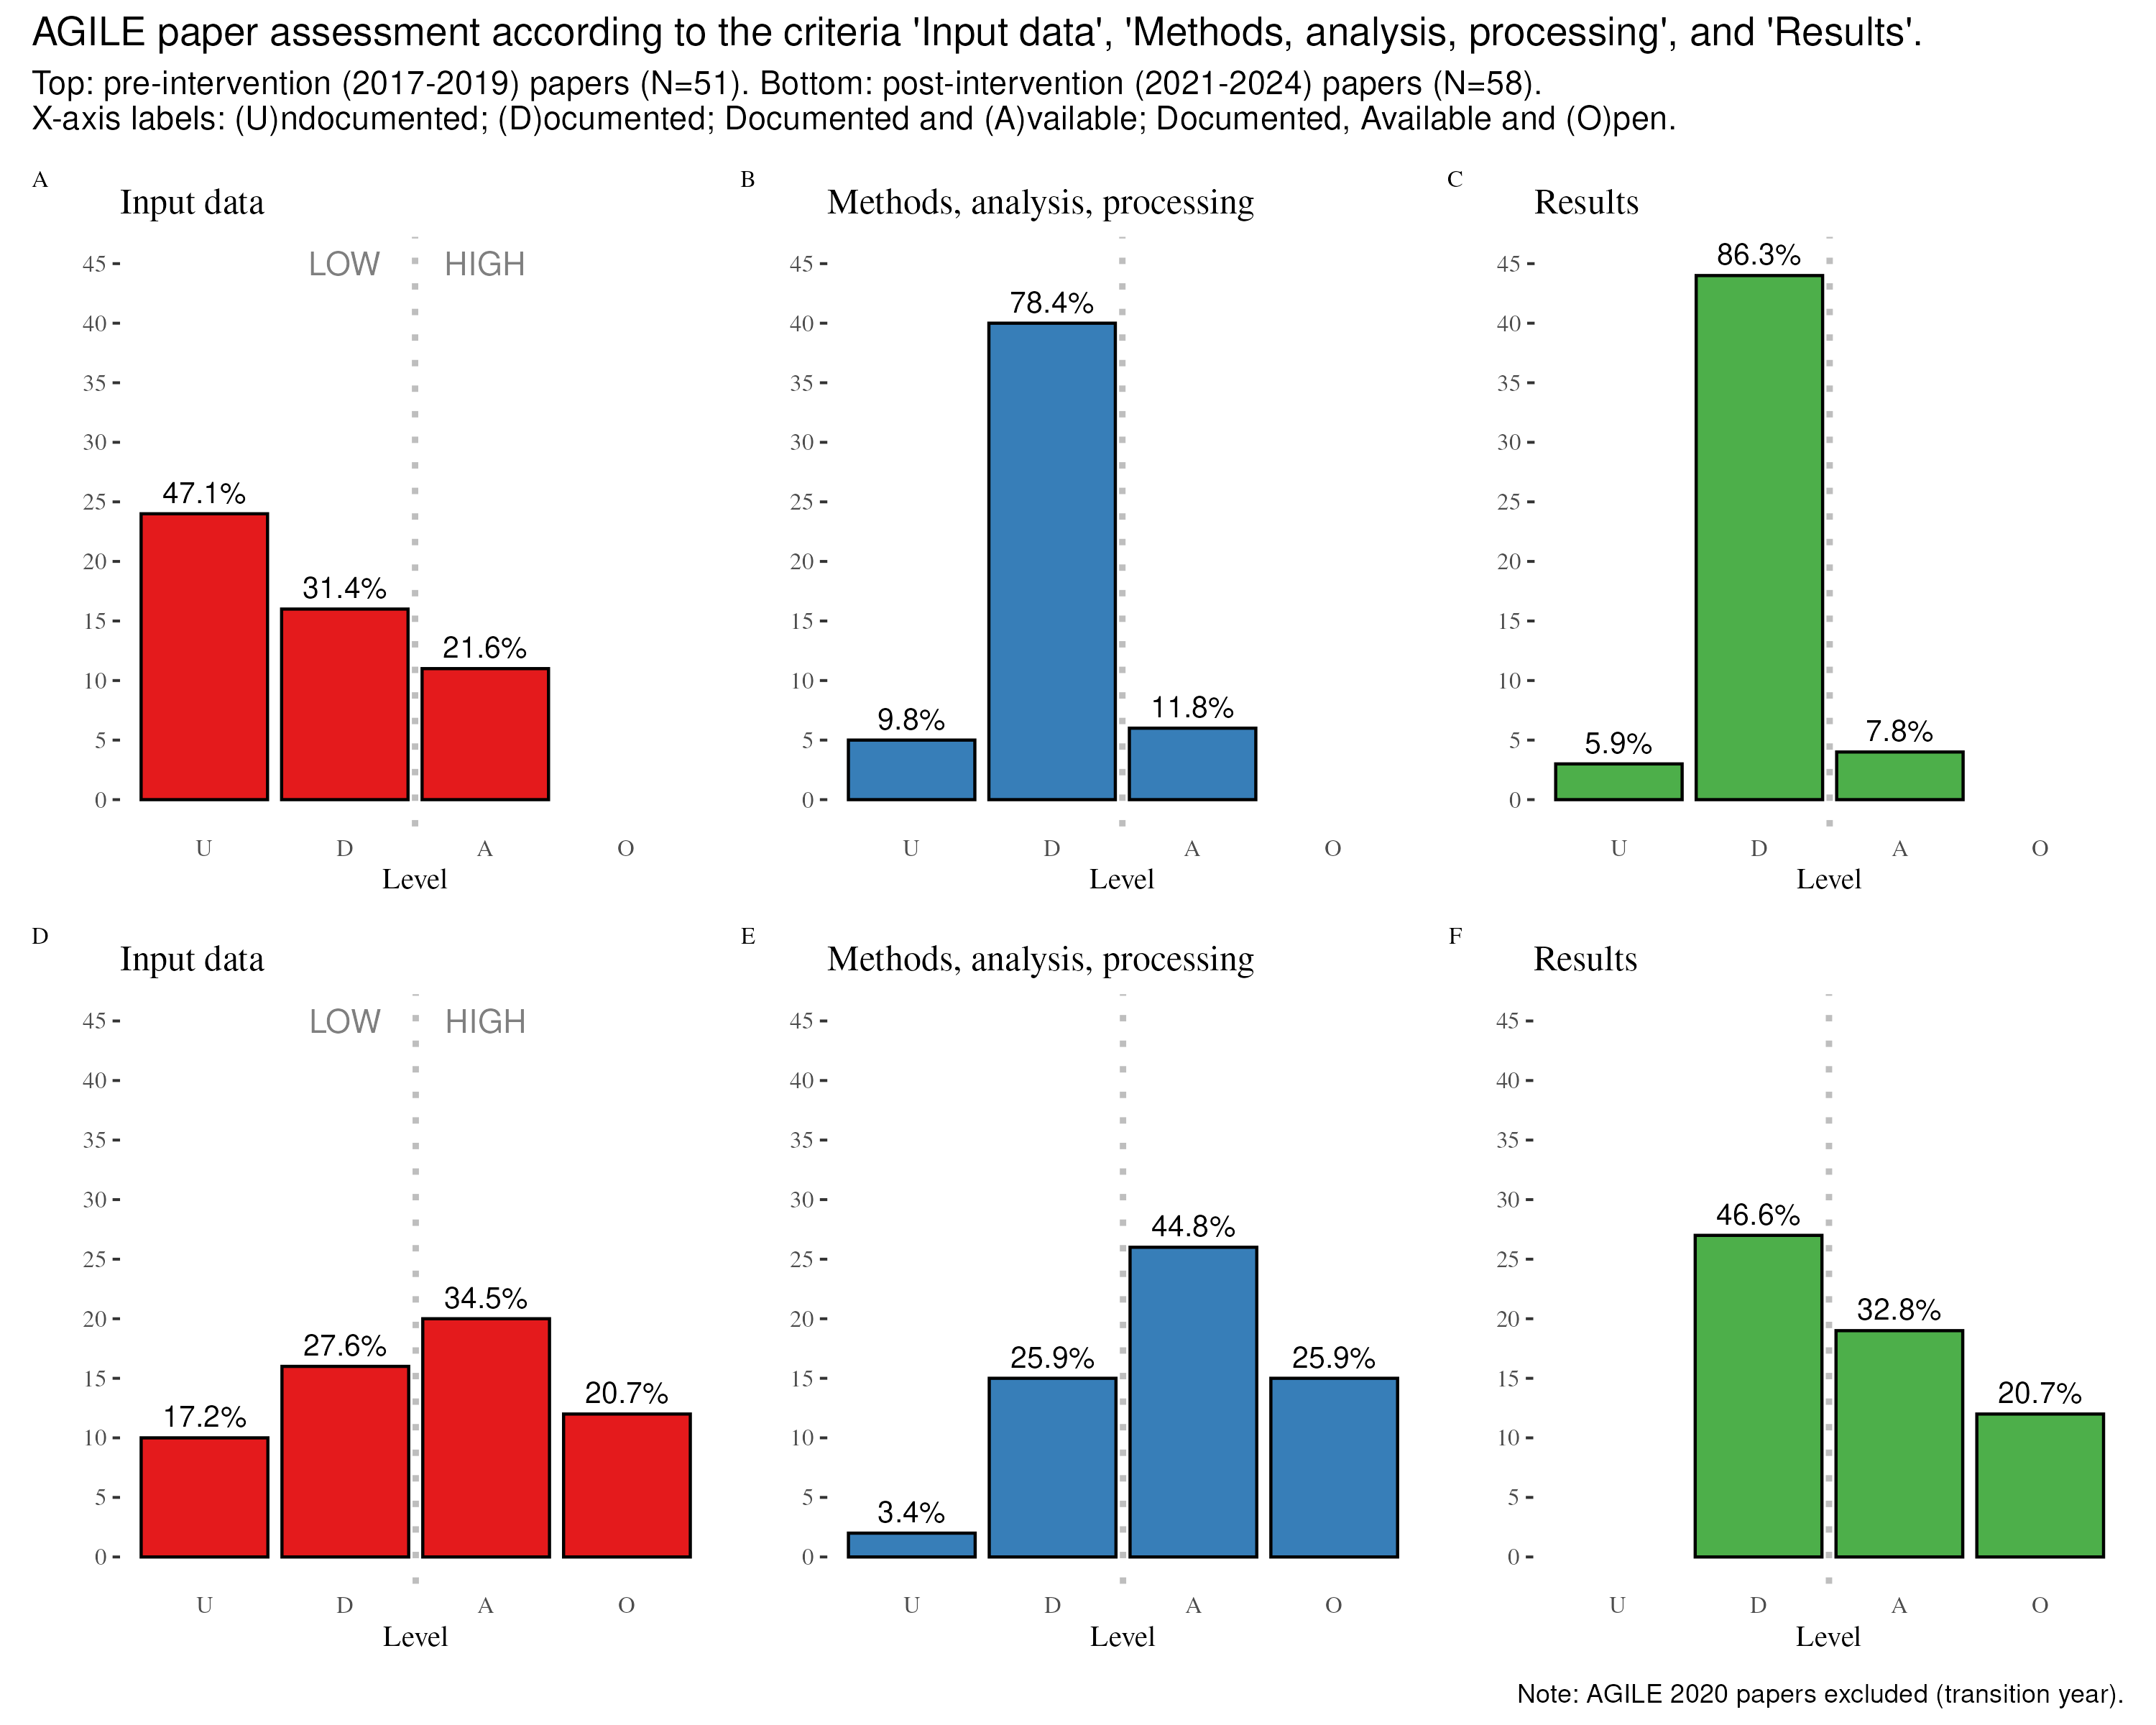
\includegraphics[width=\textwidth]{img/AGILE_pre_post.png}
\caption{Evaluation of the potential reproducibility level of AGILE papers (pre- vs post-intervention) for each criterion: \textit{Input data} (A, D), \textit{Methods, analysis, processing} (B, E), and \textit{Results} (C, F). Source: \texttt{03\_results\_reprolevels.qmd}~\cite{data}.}\label{fig:agile}
\end{figure}

The assessment results of the pre-intervention AGILE papers (Figure~\ref{fig:agile}, top) match the results of a previous study in which we evaluated the best papers of the 2010, and 2012 to 2017 AGILE conferences~\cite{nust2018}.
None of the pre-intervention AGILE papers reached the highest level of documented, available and open (from here on: Open) on any criterion.
One issue encountered in the previous study~\cite{nust2018} persists in the current larger pool of pre-intervention AGILE papers: the high proportion of papers (24, or 47.1\%) with level Undocumented for \textit{Input data}, meaning that the input datasets used in these studies were never available, and cannot even be re-created today from the information they contain.

For the pre-intervention \textit{Methods, analysis, processing} and \textit{Results} criteria, the proportion of papers with Documented level is remarkably high: 40 publications (78.4\%) and 44 (86.3\%) respectively. 
These percentages suggest that authors provide sufficient documentation in their articles for reviewers and readers to follow the presented argument and analysis. 
Our analysis deviates from the earlier review of AGILE papers~\cite{nust2018} because there are now more papers that meet the level of documented and available (from here on: Available) in the criteria of \textit{Methods, analysis, processing} and \textit{Results}, indicating a slight improvement compared to our previous study.
However, this observed difference is based on a small number of studies and so should be interpreted with caution. 

The assessment results of the post-intervention AGILE papers (Figure~\ref{fig:agile}, bottom) present a completely different picture. 
The first significant observation is that a considerable number of papers reached the highest potential reproducibility level of Open for all criteria. 
This is particularly relevant when compared to the pre-intervention AGILE papers, as this level had never been achieved on any of the criteria.
During the post-intervention period, the frequency distribution of the \textit{Input data} criterion tends to be right-skewed, implying that higher levels of potential reproducibility are reached, 
which in turn results in a greater number of assessments in the aggregate \textit{High} level.
Available is the most frequently reached level (20 papers, 34.5\%), comprising more than a third of post-intervention AGILE papers. 
Together with the 12 articles (20.7\%) labelled as Open, these two levels together (\textit{High}) represent more than 55\% of the total articles. 
This level of reproducibility ensures that the datasets used are available at the time of publication and subsequently, which represents a significant improvement to pre-intervention situation, where almost 80\% were categorised as \textit{Low}. 
However, 16 papers (27.6\%) only reached the minimum level of Documented and 10 papers (17.2\%) remained as Undocumented, indicating that there is still room for improvement when it comes to reproducing input data sets.

Similarly, the most frequently observed level in the \textit{Methods, analysis, processing} criterion during the post-intervention period was Available, which represented nearly half of the post-intervention AGILE papers (26 papers, 44.8\%). 
If we also account for the 15 papers that reached the highest level, Open, about 70\% of papers are categorised as \textit{High} in this criterion. 
The Documented level, which was the most frequent level in pre-intervention (8 out of 10 articles met this level), dropped to only a quarter of the post-intervention articles, representing a four-fold reduction, which suggests an improvement in reproducibility.

Regarding \textit{Results}, the most common potential reproducibility level remains Documented, followed by the two higher levels (Available, Open). 
While the highest two levels together only account for 7.8\% of pre-intervention AGILE articles, the percentage considerably grew to 53.5\% of post-intervention AGILE papers. 
This seven-fold increase indicates a clear improvement in reproducibility for the post-intervention AGILE articles.


\subsubsection{GIScience papers}

\begin{comment}
CARLOS: I commented this figure (GIScience_all.png) and associated text because I initially  considered all nonconceptual GIScience papers, and I should also have excluded GIScience 2021 Part I papers (actually published in 2020). 

\begin{figure}[tbh]
\centering
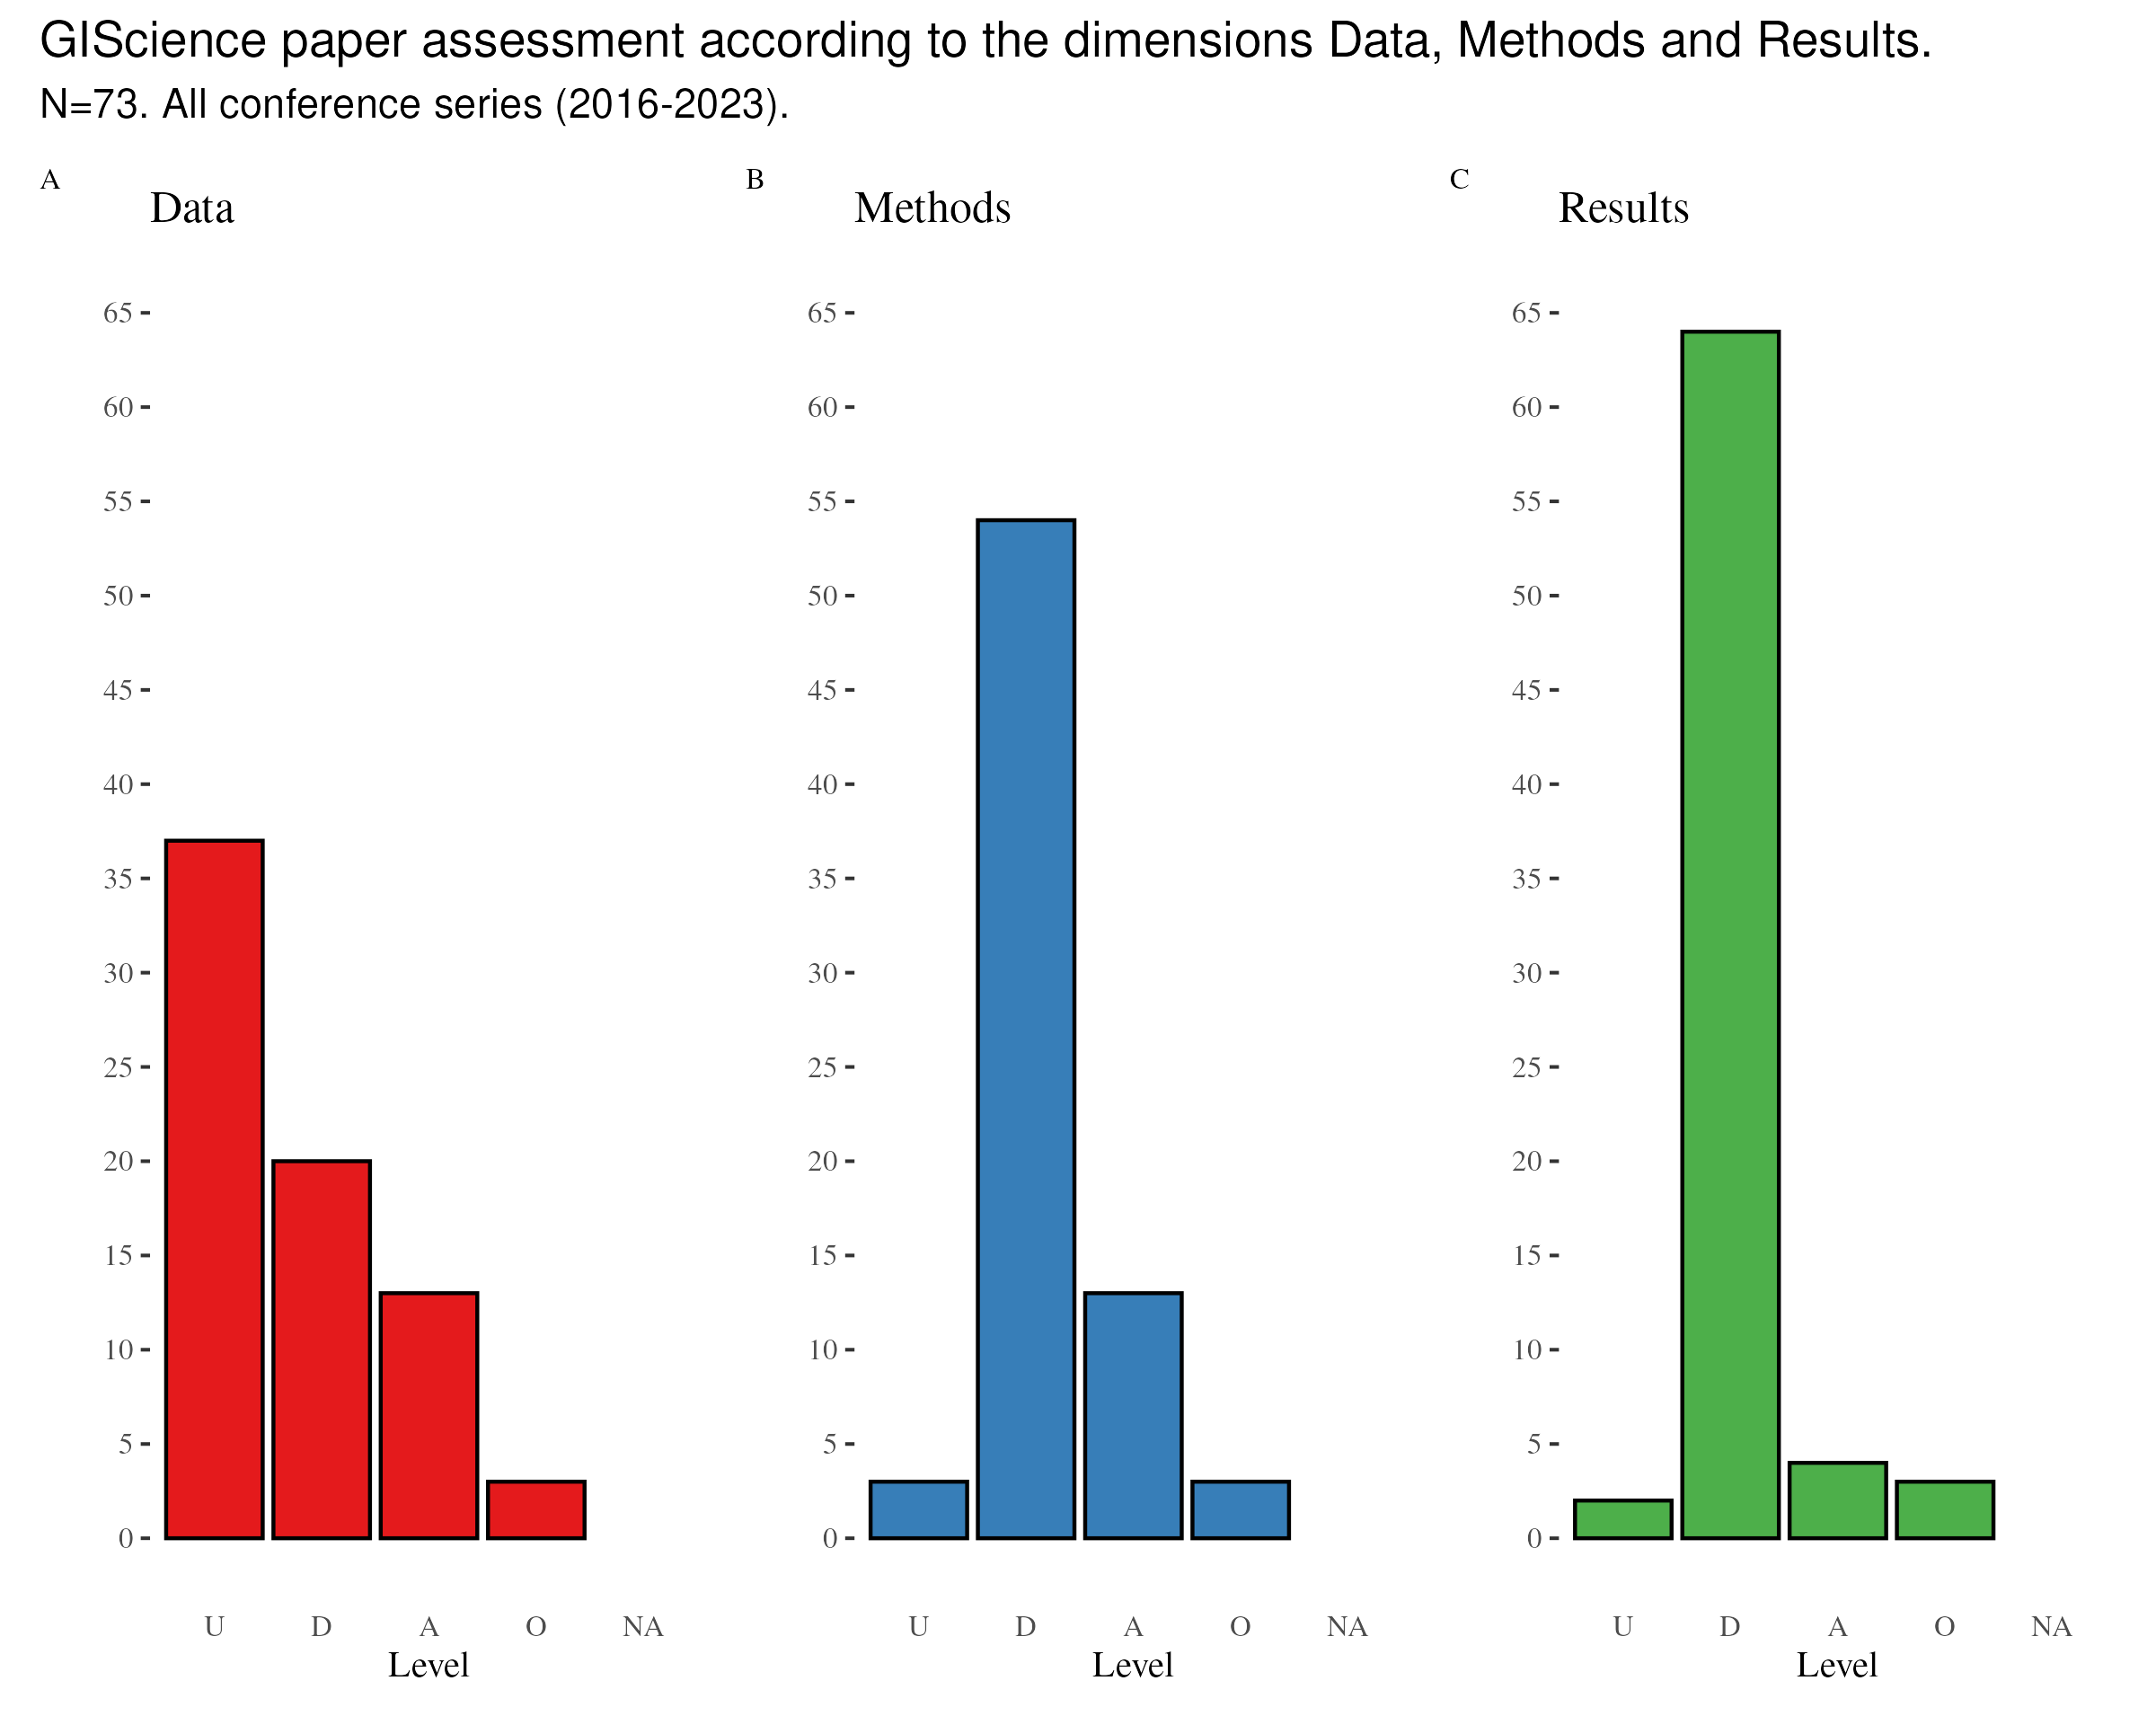
\includegraphics[width=\textwidth]{img/GIScience_all.png}
\caption{Evaluation of the reproducibility level of GIScience papers for each criterion: Data (A), Methods (B) and Results (C). Source: \texttt{03\_eligible\_papers.qmd}~\cite{data}.}\label{fig:giscience}
\end{figure}

Of the 203 non-conceptual papers (90.6\% of the total papers) that were assessed, GIScience papers represent 36\% (73/203) and AGILE papers 64\% (130/203). Figure~\ref{fig:giscience} shows the frequency of each reproducibility level for each criterion for the GIScience papers. As regards the \textit{Input Data} criterion, only three papers (4.1\%) reached the highest reproducibility level of Available and Open (O), while 13 papers (17.8\%) reached level Available (A). The number of papers with level Undocumented (U) was especially high 37 (50.7\%). These percentages reflect very well the results of a previous study focused on the GIScience conference series for a different time period (2012, 2014, 2016, and 2018 editions) and with different reproducibility reviewers~\cite{ostermann2021}. The problem identified at that time remains exactly the same for more recent conference editions: the large proportion of papers with undocumented input datasets represents a significant barrier to reproduction, as the input data are not only unavailable but also cannot be recreated from the information provided in the paper.

The \textit{Methods} and \textit{Results} criteria show a similar frequency distribution (see Figure~\ref{fig:giscience}) that is very different from that for \textit{Input Data}. Indeed, 54 publications (74\%) for \textit{Methods} and 64 (87.7\%) for \textit{Results} have level Documented. In this sense, most of the assessed GIScience papers meet the minimum standard of publication (Documented) in the methods and results criteria. All papers except two reached this level for the \textit{Results} criterion, which shows that the peer review worked as expected for almost all papers. In other words authors are concerned with making the results understandable to the reviewers, which is not always the case for the \textit{Input Data} criterion. Again, these results are very much in line with what we stated in our previous study for the \textit{Methods} and \textit{Results} criteria~\cite{ostermann2021}.
\end{comment}



Figure~\ref{fig:giscience} shows the frequency of potential reproducibility levels for each criterion for the GIScience papers.
The figure divides the GIScience conference series horizontally into two groups. 
The criteria for the pre-guidelines conferences held in 2016 and 2018 editions are in the upper row, the criteria assessments for the post-guidelines conferences held in 2021 and 2023 editions are in the lower row. 
Recall that the GIScience conference series never implemented a reproducibility review, but are nonetheless divided for comparison with the AGILE Conference.

\begin{figure}[tbh]
\centering

\includegraphics[width=\textwidth]{img/GIScience_pre_post.png}
\caption{Evaluation of the potential reproducibility level of GIScience (2016, 2018 vs 2021, 2023) for each criterion: \textit{Input data} (A, D), \textit{Methods, analysis, processing} (B, E), and \textit{Results} (C, F). Source: \texttt{03\_results\_reprolevels.qmd}~\cite{data}.}\label{fig:giscience}
\end{figure}

For the pre-guidelines GIScience papers (Figure~\ref{fig:giscience}, top), the number of papers with level Undocumented on the \textit{Input data} criterion was especially high (19, or 56\%) while none of the pre-intervention papers reached the higher end of the spectrum on that criterion. 
Indeed, the Open level was missing for all criteria. The Documented level and  Available level shared the same proportion, around 20\%, for \textit{Input data}. 
These percentages mirror the results of a previous study focused on the GIScience conference series alone and with different assessors~\cite{ostermann2021}. 
We identify the same underlying problem in the more recent conference editions: the large proportion of papers with undocumented input datasets represents a significant barrier to reproduction.
Input data are not only unavailable, the data cannot be recreated from the information provided in the paper.

The \textit{Methods, analysis, processing} and \textit{Results} criteria show a similar frequency distribution (see Figure~\ref{fig:giscience}, top) that is very different from that for \textit{Input data}. 
The same number of publications (32, or 94\%) for \textit{Methods, analysis, processing} and \textit{Results} have the Documented level. 
In this sense, most of the assessed GIScience papers meet the minimum standard of publication (i.e., Documented) in both criteria. 
All papers except two reached this level for the \textit{Results} criterion, which shows that the peer review worked as expected.
In other words, authors are concerned with making the results understandable to the reviewers, which is not always the case for the \textit{Input data} criterion. 
These results again align with earlier reproducibility reviews of GIScience articles~\cite{ostermann2021}.

Assessment results of the post-guidelines GIScience papers (Figure~\ref{fig:giscience}, bottom) show a different picture. 
First, a few post-guidelines papers achieved the highest potential reproducibility level of Open on any criterion (not necessarily in the same paper).
Still, half of the papers (12) merely reached the Undocumented level for the \textit{Input data} criterion, which represents a barrier to reproducibility.
The most frequent level (12, or 50\%) in the \textit{Methods, analysis, processing} criterion is Documented, the same as the pre-guidelines period.
However, there are some differences, as the number of papers with the Available level has increased significantly from 1 (3\%) to 9 (37.5\%).
Regarding \textit{Results}, Documented remains the most common potential reproducibility level, but the frequency distribution shows notable shifts compared to the pre-guidelines period: four papers are available (16.7\%), two are Open (8.3\%), while the Undocumented level is missing.
These changes clearly show a change towards higher reproducibility levels in the post-guidelines GIScience conference editions.


\subsubsection{Comparison between conferences}

The assessment results of the pre-intervention AGILE papers (Figure~\ref{fig:agile}, top) show similar patterns to the results of the pre-intervention GIScience conference series (Figure~\ref{fig:giscience}, top). In other words, the top rows of both figures are quite similar and show continuity with the reproducibility assessments of our previous studies in preceding years. Lower rows in both figures, however, present right-skewed distributions, favouring \textit{High} levels of potential reproducibility. Despite this overall improvement, post-intervention AGILE papers show a more pronounced shift towards the \textit{High} level across all criteria than post-guidelines GIScience papers.

To better illustrate the change after the introduction of the AGILE Guidelines between both conferences, Table~\ref{tbl:change} shows the change in absolute percentage points in potential reproducibility levels for each criterion and conference. 
For simplicity, we compare the aggregate reproducibility level \textit{High} (A, O).  
%In each horizontal bar in Figure~\ref{tbl:change} we 
To do so, we determine for each aggregated criterion whether the \textit{High} level has increased or decreased in absolute percentage points before and after the intervention. 
Positive percentage points in Table~\ref{tbl:change} indicate an improvement in reproducibility towards \textit{High} level, while negative value indicate a decrease of \textit{High} level in post-intervention (or post-guidelines) papers, suggesting no progress towards reproducibility in a given criterion. 
Overall, the improvements are very significant for AGILE compared to GIScience across all criteria, but are particularly notable with respect to \textit{Input data} criterion, given that GIScience post-intervention papers do not improve on that criterion.

%\begin{figure}[tbh]
%\centering
%
\includegraphics[width=\textwidth]{img/GIScience_AGILE_delta.png}
%\caption{Change in absolute percentage points of the potential reproducibility level of both conference papers (pre- vs post-intervention). Source: \texttt{04\_results\_reprolevels.qmd}~\cite{data}.}\label{fig:change}
%\end{figure}


% Created automatically with gt::as_latex() 

\begin{table}
\centering
\begin{tabular*}{\linewidth}{@{\extracolsep{\fill}}lcc}
\toprule
\textit{High} level per criterion & GIScience & AGILE \\ 
\midrule\addlinespace[2.5pt]
Input data  & -3.9 & 33.6 \\ 
Methods, analysis, processing  & 42.9 & 58.9 \\ 
Results  & 25.0 & 45.6 \\ 
\bottomrule
\end{tabular*}
\caption{Absolute change in percentage points between GIScience vs AGILE after the intervention for the \emph{High} level. Source: \texttt{03\_results\_reprolevels.qmd}~\cite{data}.}\label{tbl:change}
\end{table}


\subsection{Hypothesis testing}
\label{sec:results:hypothesis}

\subsubsection{Changes in AGILE papers (Hypothesis A)}

Our Null-Hypothesis A is that there is no difference in the level of potential reproducibility of AGILE papers between pre-intervention papers (2017, 2018, 2019) and post-intervention papers (2021, 2022, 2023). 
%The alternative hypothesis A, in case we reject our null hypothesis is that the level of potential reproducibility has indeed changed after the intervention.

\begin{table}
\begin{tabular}{lrrrrrrrr}
\toprule
 & \multicolumn{2}{c}{Mean} & \multicolumn{2}{c}{Median} & \multicolumn{2}{c}{Mode} & U1-Stat & P-value \\
 & pre & post & pre & post & pre & post &  &  \\
\midrule
Input data & 0.745 & 1.586 & 1 & 2 & 0 & 2 & 804.000 & <0.001 \\
Methods, analysis, processing & 1.020 & 1.931 & 1 & 2 & 1 & 2 & 565.000 & <0.001 \\
Results & 1.020 & 1.741 & 1 & 2 & 1 & 1 & 740.000 & <0.001 \\
\bottomrule
\end{tabular}
\caption{Descriptive statistics and Mann-Whitney-U scores values for AGILE group before and after intervention, per criterion. Source: \texttt{04\_results\_hypotheses.ipynb}~\cite{data}.}
\label{tab:mannwhitney_agile}
\end{table}

Table~\ref{tab:mannwhitney_agile} shows a statistically significant change in potential reproducibility for all three criteria at the chosen significance level of 0.01.
We therefore reject the null hypothesis for \textit{Input data}, \textit{Methods, analysis, processing}, and \textit{Results} criteria and state that there was a significant change in potential reproducibility of papers published at the AGILE conference series after the introduction of the AGILE Guidelines. 
The descriptive statistics indicate that this change was an increase: Mode, median, and mean ranks all have increased, but the increase to modes and medians of rank 2 is especially meaningful, because the corresponding level of Available means that all required materials are available for reproduction at the time of publication. 

\subsubsection{Changes in GIScience papers (Hypothesis B)}

Our Null-Hypothesis B postulates a change in the level of potential reproducibility of GIScience papers between GIScience pre- (2016 and 2018) and post-intervention (2021 and 2023) papers. 
The alternative hypothesis is that the level of potential reproducibility has \emph{not} changed after the intervention.

\begin{table}
\begin{tabular}{lrrrrrrrr}
\toprule
 & \multicolumn{2}{c}{Mean} & \multicolumn{2}{c}{Median} & \multicolumn{2}{c}{Mode} & U1-Stat & P-value \\
 & pre & post & pre & post & pre & post &  &  \\
\midrule
Input data & 0.647 & 0.750 & 0 & 0 & 0 & 0 & 389.000 & 0.747 \\
Methods, analysis, processing & 1.000 & 1.500 & 1 & 1 & 1 & 1 & 242.000 & <0.001 \\
Results & 0.941 & 1.333 & 1 & 1 & 1 & 1 & 288.000 & 0.002 \\
\bottomrule
\end{tabular}
\caption{Descriptive statistics and Mann-Whitney-U scores values for GIScience group before and after intervention, per criterion. Source: \texttt{04\_results\_hypotheses.ipynb}~\cite{data}.}
\label{tab:mannwhitney_giscience}
\end{table}

Table~\ref{tab:mannwhitney_giscience} presents the descriptive statistics for the conducted tests. 
It shows that for \textit{Input data}, there was no statistically significant change in potential reproducibility at the chosen significance level of 0.01. For \textit{Methods, analysis, processing} and \textit{Results}, there were statistically significant changes (increases) in potential reproducibility at the chosen significance level of 0.01.
We therefore reject the original hypothesis only for the \textit{Input data} criterion and conclude that the potential reproducibility of data has not increased, but \textit{Methods, analysis, processing} and \textit{Results} have changed (increased).

While the mean ranks have increased slightly, there is no change in mode or median, indicating that while overall reproducibility has improved, most papers still fall short of reaching the level Available. 

\subsubsection{Comparison between conferences (Hypothesis C)}

Hypothesis C postulates that the development of potential reproducibility of AGILE papers over time is not different from that of GIScience papers: neither in direction nor in strength.

The analysis shows that the rank-biserial correlations are negative for all tests, indicating better ranks in the second (post-intervention) group (see Table~\ref{tab:rankbiserial}).
For every tested dimension, the scores and thus effect sizes are larger for AGILE than for GIScience.

\begin{table}
\centering
\begin{tabular}{lrcrr}
\hline
Criterion & AGILE & GIScience \\
\hline
Input data & -0.456 & -0.047 \\
Methods, analysis, processing & -0.618 & -0.407 \\ 
Results & -0.500 & -0.294\\ 
\hline
\end{tabular}
\caption{Rank-Biserial values for AGILE and GIScience groups before and after intervention, per criterion. Source: \texttt{04\_results\_hypotheses.ipynb}~\cite{data}.}
\label{tab:rankbiserial}
\end{table}


The analysis of the log odds ratios in Table~\ref{tab:oddsratios} shows a similar pattern: both AGILE and GIScience have improved, i.e., the likelihood of a paper being reproducible is higher in the post-intervention group. 
For the \textit{Input data} criterion, AGILE shows better odds than GIScience, which has even a slightly negative but statistically not significant value. 
However, for GIScience papers the improvements for \textit{Methods, analysis, processing} and \textit{Results} are larger than for AGILE, albeit with a larger confidence interval. 
This can be interpreted as higher but at the same time more varied improvement.
Note that the lower bound of the confidence interval for \textit{Results} for GIScience is even negative, which can also be a reflection of the low frequency of highly reproducible GIScience papers in the pre-intervention group.

\begin{table}
\begin{tabular}{lrrrrrrrr}
\toprule
 & \multicolumn{4}{c}{AGILE} & \multicolumn{4}{c}{GIScience} \\
 & OR & CI lower & CI upper & P-value & OR & CI lower & CI upper & P-value \\
\midrule
Input data & 1.499 & 0.389 & 2.608 & <0.001 & -0.260 & -2.044 & 1.525 & 0.710 \\
Methods, ... & 2.895 & 1.552 & 4.239 & <0.001 & 3.329 & 0.510 & 6.149 & <0.001 \\
Results & 2.602 & 1.099 & 4.105 & <0.001 & 3.121 & -0.744 & 6.986 & 0.005 \\
\bottomrule
\end{tabular}
\caption{Odds ratios (OR), upper and lower 95\% confidence intervals (CI upper/lower) and Fischer exact P-Values for AGILE and GIScience groups before and after intervention, per criterion. Source: \texttt{04\_results\_hypotheses.ipynb}~\cite{data}.}
\label{tab:oddsratios}
\end{table}

The rank-biserial correlations, the odds rations, and a comparison of the descriptive statistics support the argument that there has been a \emph{general increase in potential reproducibility in the research domain of GIScience} over the study period, and that this increase is \emph{larger in relative terms and absolute ranks for papers published at the AGILE conference series}.

\subsection{Assessment disagreements}
\label{sec:results:assessmentprocess}

As introduced in Section~\ref{sec:methods:assessment:disagreement}, we categorised disagreements based on the assessors’ annotations and assessment scores: no disagreement, borderline conceptual paper, annotation inconsistencies, uncertain assessment, and significant disagreement. Here, we consider the total number of papers (224), as the transition year provides useful data for the particular analysis of assessment disagreement between assessors.

Independent assessors infrequently agreed about the potential reproducibility of the papers they commonly evaluated.
Assessors agreed on the potential reproducibility of papers in only 28\% of the cases, while disagreements occurred in over 70\% of cases (see Table~\ref{tab:all_discrepances}). 
We did not include a plan to analyse assessor agreement in our preregistration because we did not expect to see such high rates of assessor disagreement; considerations about the assessment process were not initially addressed. 
However, our finding is consistent with previous studies~\cite{kedron2025, konkol_computational_2019}, which highlight the heterogeneity of perceptions regarding reproducibility and replicability, often shaped by an assessor’s expertise, disciplinary background, and subjective interpretation. 
Evaluating the reproducibility of a scientific paper is inherently complex and nuanced, and is influenced by individual experience. 
The high rate of disagreement we observed aligns with previously identified disagreement causes, reflecting patterns reported in earlier reproducibility studies~\cite{nust2018, ostermann2021}.
   

\begin{table}
\centering
\begin{tabular}{lrcrr}
\hline
Disagreement type & \# & \% \\
\hline
Uncertain assessment & 100 & 44.6\% \\
No disagreement & 63 & 28.1\% \\ 
Significant disagreement & 42 &  18.8\% \\ 
Borderline conceptual paper & 14 & 6.2\% \\ 
Annotation inconsistencies & 5 & 2.2\% \\ 
\textbf{Total} &  \textbf{224} & \\
\hline

\end{tabular}
\caption{Distribution of disagreement types. Source: \texttt{05\_results\_assessprocess.qmd}~\cite{data}.}
\label{tab:all_discrepances}
\end{table}

After excluding cases of ``no disagreement'', we found that 53\% of assessor discrepancies categorised as ``borderline conceptual paper'', ``uncertain assessment'', and ``annotation inconsistencies'' were due to divergent interpretations of the assessment criteria. 
This finding suggests that refining and clarifying the Assessment Protocol would likely reduce such inconsistencies. 
In contrast, ``significant disagreements'' (approximately 20\%) were related to deeper issues with the papers and the Assessment Protocol. 
Specifically, such disagreements were often related to insufficient detail in the assessed papers, which was compounded by imprecise guidance in the Assessment Protocol document. 
These cases underscore the difficulty of attributing discrepancies to a single factor, as they often arise from a combination of unclear reporting and interpretive variability.

Analysis across the two conferences revealed no remarkable differences in the overall distribution of disagreement types. 
AGILE papers exhibited a slightly higher proportion of ``significant disagreements'' (20.5\% in AGILE vs. 15.5\% in GIScience), while GIScience papers showed a slightly higher proportion of ``borderline conceptual paper'' (5.5\% in AGILE vs 7.7\% in GIScience) and ``no disagreement'' (27.4\% in AGILE vs. 29.5\% in GIScience). 
A plausible explanation is that GIScience papers tend to be more theory-oriented, whereas AGILE contributions are generally application-driven. 
Theoretical papers, which typically involve fewer computational components and datasets, may be easier to assess based on our reproducibility criteria, thus reducing the number of ambiguous cases. 
In contrast, applied research papers typically involve more complex methodological and code- and data-related components, which can increase the potential for disagreement in assessment. 
Therefore, the nature of the research -- specifically, the relative prevalence of theoretical versus applied research -- could be a contributing factor to the observed differences in disagreement types between the two conferences. 
While the differences are modest, they underscore the importance of tailoring assessment protocols (and tools) to the characteristics of the research community being evaluated.

\begin{figure}[tbh]
\centering
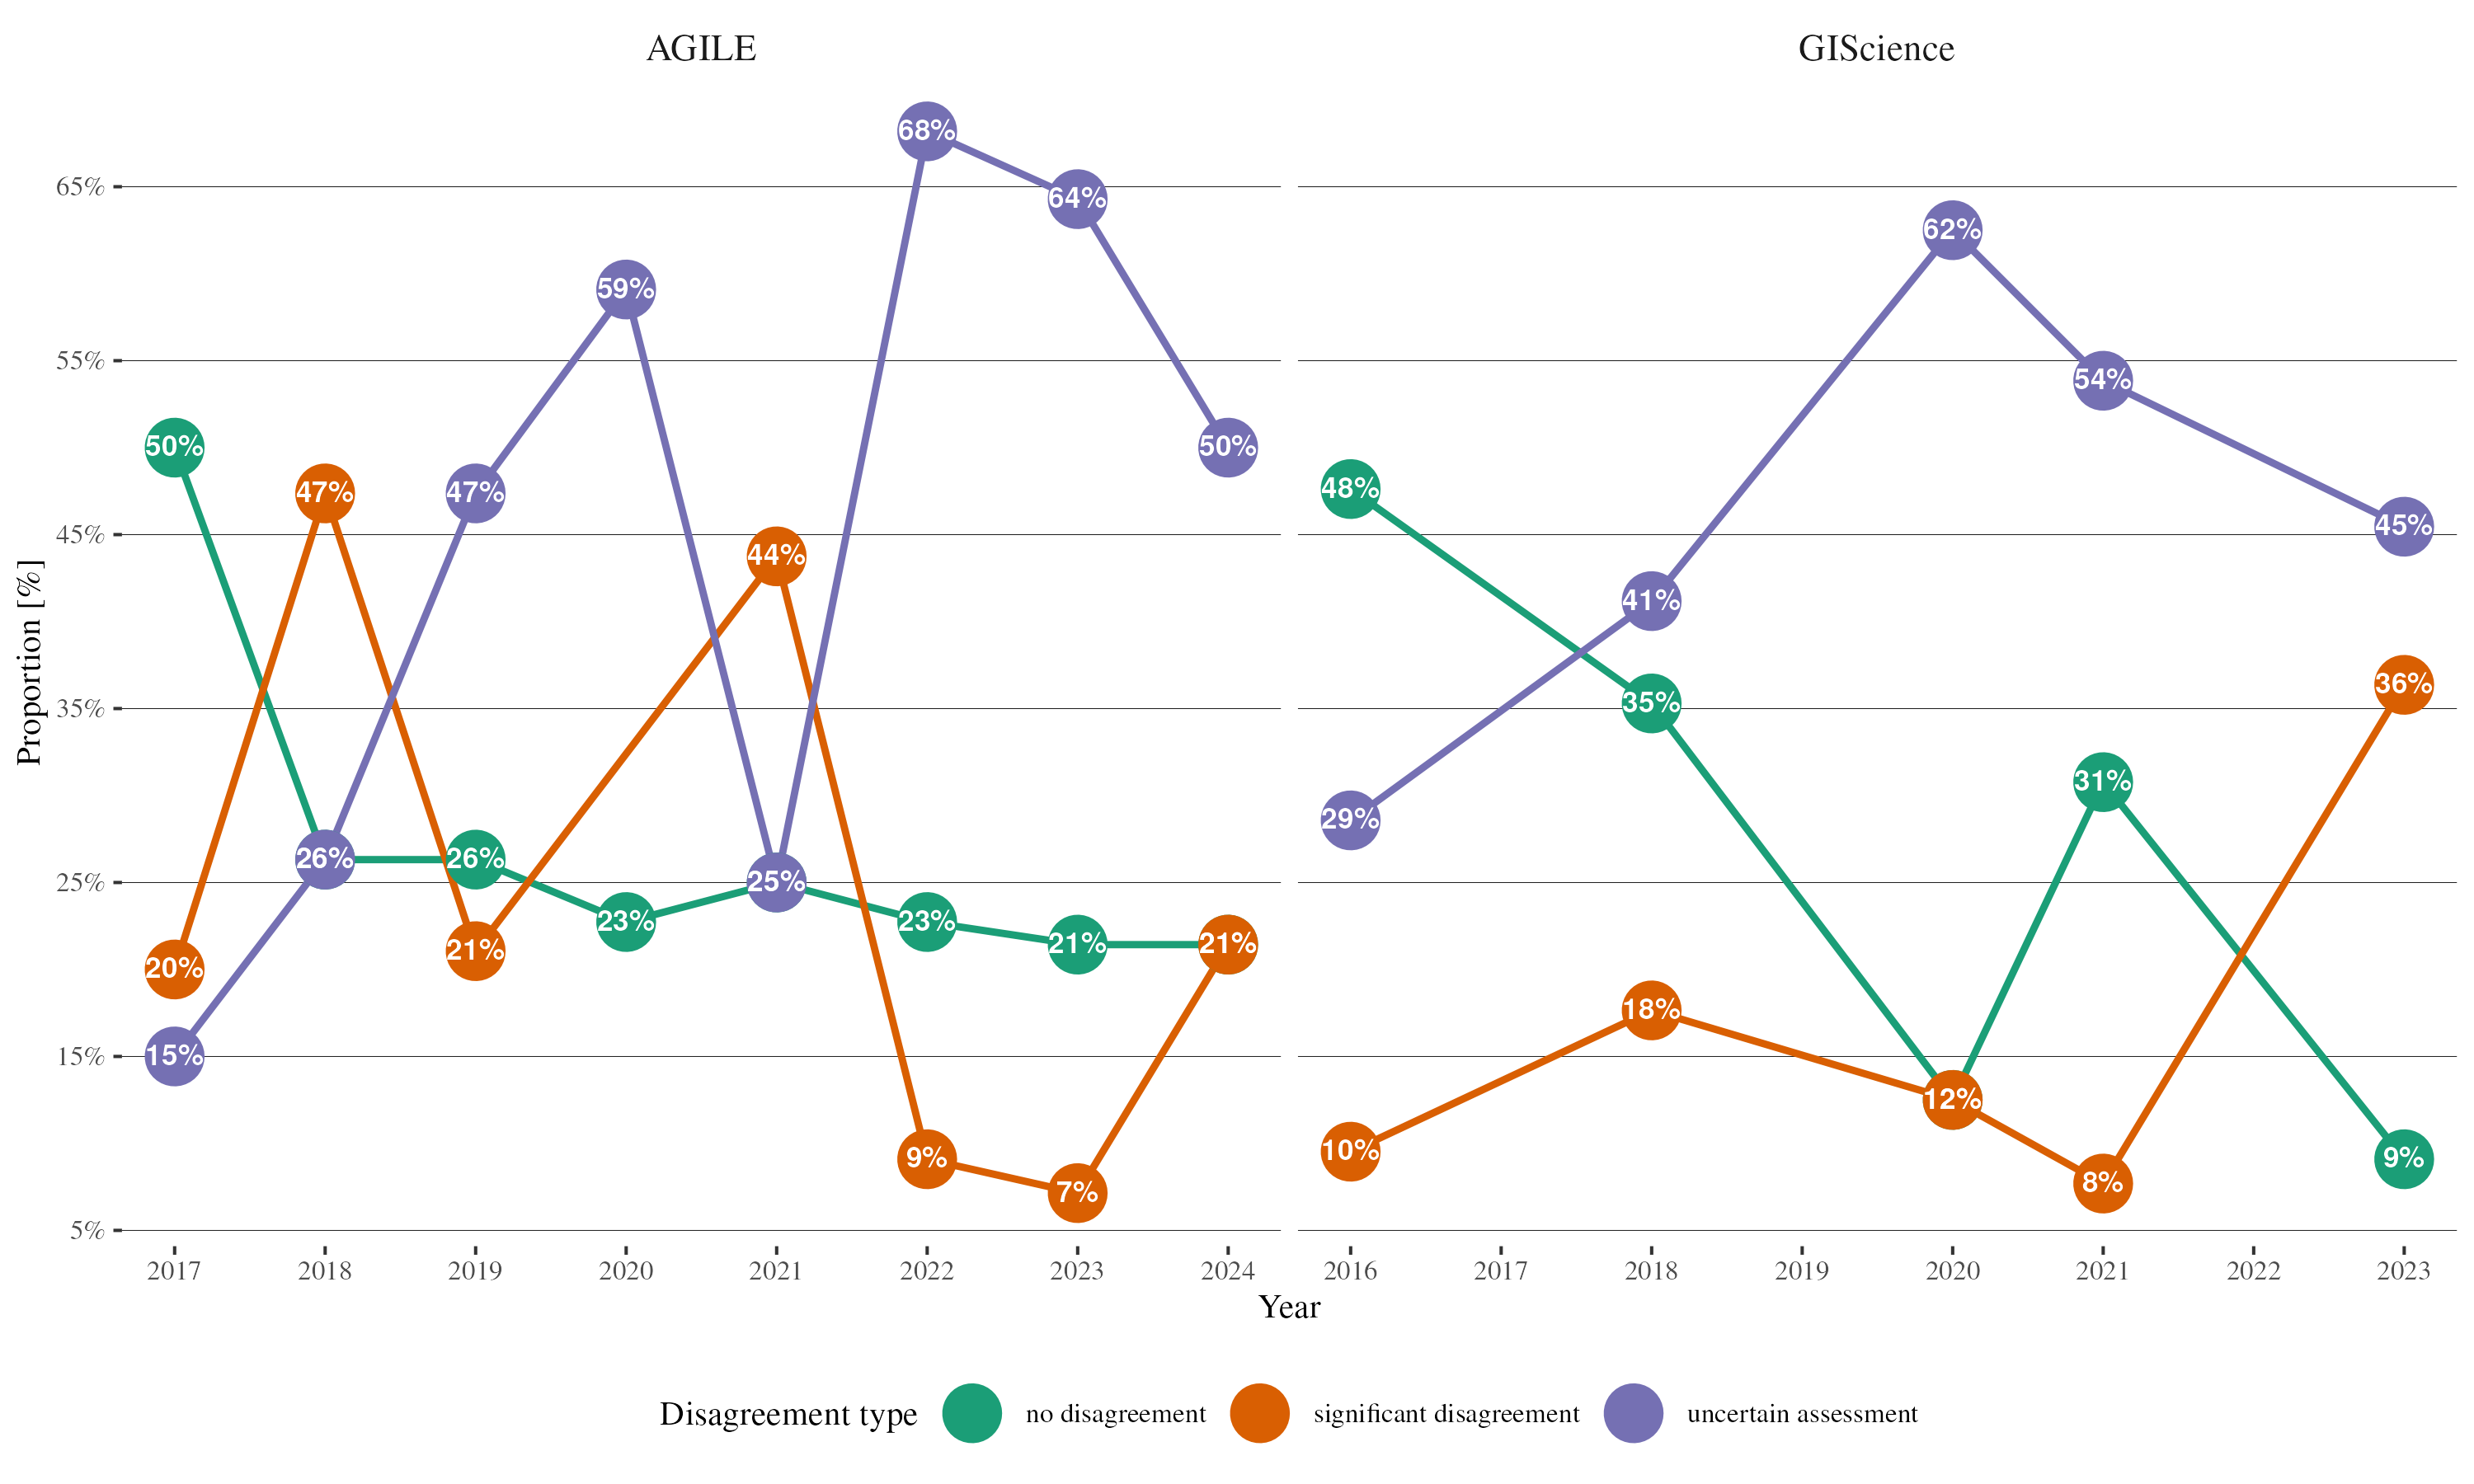
\includegraphics[width=\textwidth]{img/top3_disagr.png}
\caption{Distribution of 3-top disagreement types per conference and year. Source: \texttt{05\_results\_assessprocess.qmd}~\cite{data}.}\label{fig:top3_disgr}
\end{figure}

Looking into the discrepancies types over years, ``borderline conceptual paper'' disagreements follow similar trend in both conferences; They are practically non-existent in recent years, while more disagreements of this type occurred for the first year of the series (AGILE 2017, GIScience 2016). 
Focusing on the top 3 disagreement types in Figure~\ref{fig:top3_disgr}, we observe that the frequency of ``no disagreement'' was lower in the more recent years, reaching its lowest percentage in the final year of the series for both conferences, suggesting that reaching consensus among assessors was much easier in the earlier years of the series (AGILE 2017, GIScience 2026, GIScience 2018) than in the later years. 
This observation may be attributed to two factors. 
First, authors have increasingly adopted best practices for documenting research resources, a practice less common in articles published in earlier conferences. 
This historical omission likely resulted in a higher frequency of past studies being classified with lower reproducibility levels (e.g. undocumented). 
Second, the increasing number of computational papers submitted to recent conference editions may make it more challenging for assessors to reach a complete consensus on all assessment criteria. For ``uncertain assessment'' and ``significant disagreement'' together, it is hard to interpret them. 
A pattern is visible over the last three conference editions: From a maximum peak (AGILE 2022, GIScience 2021 Part I -  published in 2020), percentage of ``uncertain assessment'' decreases while that of ``significant disagreement'' increases for both conferences. 
However, the increase in ``significant disagreement'' is greatest at the latest GIScience 2023 conference. 
This may be partly due to the lack of explicit reproducibility guidelines for GIScience authors, as the number of computational papers at recent GIScience conferences has notably increased.

% Created automatically with gt::as_latex() 
\begin{table}
\centering
\begin{tabular*}{\linewidth}{@{\extracolsep{\fill}}clcclcclcc}
\toprule
 & \multicolumn{3}{c}{\textbf{Input data}} & \multicolumn{3}{c}{\textbf{Methods, \ldots{}}} & \multicolumn{3}{c}{\textbf{Results}} \\ 
\cmidrule(lr){2-4} \cmidrule(lr){5-7} \cmidrule(lr){8-10}
\emph{Conf Series} & \emph{Disagr?} & \emph{\#} & \emph{\%} & \emph{Disagr?} & \emph{\#} & \emph{\%} & \emph{Disagr?} & \emph{\#} & \emph{\%} \\ 
\midrule\addlinespace[2.5pt]
AGILE & no & 23 & 35.4\% & no & 46 & 70.8\% & no & 36 & 55.4\% \\ 
{AGILE} & {yes} & {42} & {64.6\%}\textsuperscript{\textit{1}} & {yes} & {19} & {29.2\%}\textsuperscript{\textit{2}} & {yes} & {29} & {44.6\%} \\ 
GIScience & no & 7 & 20.0\% & no & 24 & 68.6\% & no & 28 & 80.0\% \\ 
GIScience & yes & 28 & 80.0\%\textsuperscript{\textit{1}} & yes & 11 & 31.4\% & yes & 7 & 20.0\%\textsuperscript{\textit{3}} \\ 
\bottomrule
\end{tabular*}
\begin{minipage}{\linewidth}
\textsuperscript{\textit{1}}Higher percentage of disagreements in both conferences.\\
\textsuperscript{\textit{2}}Lower percentage of disagreements at the AGILE conference.\\
\textsuperscript{\textit{3}}Lower percentage of disagreements at the GIScience conference.\\
\end{minipage}
\caption{Distribution of ``uncertain assessment'' (N=100) per conference and criterion. Source: \texttt{05\_results\_assessprocess.qmd}~\cite{data}.}\label{tbl:uncertain_disgr}
\end{table}

% Created automatically with gt::as_latex() 
\begin{table}
\centering
\begin{tabular*}{\linewidth}{@{\extracolsep{\fill}}clcclcclcc}
\toprule
 & \multicolumn{3}{c}{\textbf{Input data}} & \multicolumn{3}{c}{\textbf{Methods,\ldots{}}} & \multicolumn{3}{c}{\textbf{Results}} \\ 
\cmidrule(lr){2-4} \cmidrule(lr){5-7} \cmidrule(lr){8-10}
\emph{Conf Series} & \emph{Disagr?} & \emph{\#} & \emph{\%} & \emph{Disagr?} & \emph{\#} & \emph{\%} & \emph{Disagr?} & \emph{\#} & \emph{\%} \\ 
\midrule\addlinespace[2.5pt]
AGILE & no & 6 & 20.0\% & no & 9 & 30.0\% & no & 13 & 43.3\% \\ 
{AGILE} & {yes} & {24} & {80.0\%}\textsuperscript{\textit{1}} & {yes} & {21} & {70.0\%} & {yes} & {17} & {56.7\%}\textsuperscript{\textit{2}} \\ 
GIScience & no & 3 & 25.0\% & no & 5 & 41.7\% & no & 5 & 41.7\% \\ 
GIScience & yes & 9 & 75.0\%\textsuperscript{\textit{1}} & yes & 7 & 58.3\%\textsuperscript{\textit{3}} & yes & 7 & 58.3\%\textsuperscript{\textit{3}} \\ 
\bottomrule
\end{tabular*}
\begin{minipage}{\linewidth}
\textsuperscript{\textit{1}}Higher percentage of disagreements in both conferences.\\
\textsuperscript{\textit{2}}Lower percentage of disagreements at the AGILE conference.\\
\textsuperscript{\textit{3}}Lower percentage of disagreements at the GIScience conference.\\
\end{minipage}
\caption{Distribution of ``significant disagreement'' (N=42) per conference and criterion. Source: \texttt{05\_results\_assessprocess.qmd}~\cite{data}.}\label{tbl:significant_disgr}
\end{table}

A similar pattern emerges when looking into the two most frequent disagreements -- ``uncertain assessment'' and ``significant disagreement''. Across both conferences, the \textit{Input data} criterion consistently accounts for the largest proportion of uncertain assessments when analysing individual scores (Table~\ref{tbl:uncertain_disgr}). In other words, assessors most often disagreed on \textit{Input data}. While uncertain disagreement may stem from subjective interpretations of the Assessment Protocol, the \textit{Input data} criterion clearly remains the most contentious. Therefore, improving guidelines are essential to help reviewers and readers evaluate input datasets more clearly and to help authors describe less ambiguously.

Likewise, when looking at significant disagreements (Table~\ref{tbl:significant_disgr}), the \textit{Input data} criterion again accounts for the highest proportion of major disagreements, regardless of the conference. It is important to note that the \textit{Methods, analysis, processing} criterion closely followed the \textit{Input data}, especially for AGILE papers (70\%), as a source of significant discrepancies. While data were the single most prevalent cause of discrepancies when analysing uncertain assessments, all criteria, but especially \textit{Input data} and \textit{Methods, analysis, processing}, are essential to understanding the causes behind significant discrepancies.


%TODO (if possible/relevant):
% - Improve current dimensions/indicators (Data, methods, etc) or suggest new ones as proxies for better assessing the level of reproducibility of a paper without performing a real reproduction of the paper  
% - ways to improve Assesment Protocol document and, consequently, the AGILE Guidelines document
% - Relate common causes of disagreement to those identified in other studies.  


\section{Discussion}

\subsection{Development of potential reproducibility}

The analysis of our data clearly shows an increase in potential reproducibility that coincides with the introduction of the AGILE Guidelines. The potential reproducibility of publications in both conference series during the 2010s was generally low, but especially low for the \textit{Input data} criterion. In the past five years, a positive trend toward higher levels of potential reproducibility was observed in both conferences, but AGILE saw a greater absolute change than GIScience and also had the higher overall (average) potential reproducibility. Whether this is due to the introduction of the AGILE Guidelines and the reproducibility reviews is open for interpretation.
We consider the evidence for such an interpretation to be strong and supported by our statistical testing. 

However, our data, especially Figure~\ref{fig:giscience}, which shows the distribution of reproducibility levels among pre- and post-guidelines GIScience articles, and Table~\ref{tbl:change}, which shows the absolute percentage point change in potential reproducibility, demonstrates a trend toward higher reproducibility levels (\textit{High}) in the post-guidelines GIScience papers as well. This trend is likely to continue, and the inclusion of more recent GIScience papers (from 2025 onwards) could show a further increase. This overall trend may be partly due to greater awareness of reproducibility within the research community, as confirmed by a recent survey in the fields of GIScience and Geography~\cite{kedron2025}. 

Another possible factor could be an overlap in the community (in terms of authors, reviewers, and scientific program committee), which could lead to a certain informal spill-over effect. 
For example, both conferences share a portion of the contributing authors~\cite{ostermann2021}:
If we look in detail into the two GIScience papers that reached level Open on all criteria \cite{ostermann2021,hildemann2023}, one author of the first paper had previously published in the AGILE conference series after the intervention~\cite{shi2023, Janowicz2022}, while the second paper ``Reproducible Research and GIScience: . . .'' was actually co-authored by authors of this study. Therefore, the indirect transfer of the AGILE Guidelines to some GIScience articles is plausible due to shared authors between the two conferences, who were strongly committed to the AGILE Guidelines. 
We consider that a more systematic investigation of authorship patterns with respect to both conference series is beyond the scope of this article, but we believe it would certainly be a valuable additional step. 

We recognise that assessing the potential reproducibility of an article without actually reproducing the study itself is only an indicator (or \textit{preproducibility}~\cite{stark2018before}). In this context, a valuable next step would be to examine the actual reproducibility of the published papers to confirm that a high level of potential reproducibility of an article aligns with successful reproduction. Obviously, this task would require reviewing and reproducing the computational workflows in a manner similar to an AGILE reproducibility review or a CODECHECK. Despite it is out of scope in this article, we took the AGILE reproducibility badge as a proxy: we compared the potential reproducibility of our assessment with the actual reproductions of AGILE papers reported during the 2021-2024 period by the Reproducibility Committee of the AGILE conference series. 

Figure~\ref{fig:sankey} shows that the level of potential reproducibility is a fairly good indicator of actual reproducibility, because almost all of the AGILE papers with high potential reproducibility earned a reproducibility badge after the reproducibility review.  
For this analysis, we group the papers into one of three groups, based on their potential reproducibility levels for the three criteria: \textit{All High}, \textit{All Low}, and \textit{High/Low}. 
For All High, a paper has to score Available or Open in all criteria, while only Undocumented or Documented levels for all criteria result in All Low. 
A High/Low rating represents a combination of any UDAO level in any criteria. 
Note that All High (or All Low) is not the same as High (or Low) described earlier. 
Of the 58 AGILE post-intervention papers in Figure~\ref{fig:sankey}, 43 earned the reproducibility badge and 15 did not. 
What stands out about this figure is that when an article received an All High rating, that article was successfully reproduced (in part or in full), as evidenced by the badge.
%Of the articles with a badge, 22 (51\%) received All High rating and 19 (22\%) High/Low. On the contrary, only 2 papers without badge (13\%) reached All High, 3 (20\%) High/Low, and 10 (67\%) received All Low rating. 
This supports the idea that if an article receives high levels of potential reproducibility (either All High or High/Low ratings) according to our reproducibility rubric, then this rubric is a good indicator of whether an article has a sufficient basis to be successfully reproduced later.

\begin{figure}[tbh]
\centering

\includegraphics[width=\textwidth]{img/AGILE_sankey_year.png}
\caption{Potential reproducibility levels as indicators of reproduction: \texttt{06\_discussion.qmd}~\cite{data}.}\label{fig:sankey}
\end{figure}

%Again, we hope that this study might be a motivation for another research group or a graduate student assignment to pick this up.

Is it then ``mission accomplished'' for the GIScience domain as a whole? 
While the improvements are certainly noteworthy and very encouraging, our investigation also showed that level of Available for \textit{Input data}, \textit{Methods, analysis, processing}, and \textit{Results} is often insufficient a few years after publication, because links to projects or code/data repositories, for example, may become unavailable for various reasons in the medium to long term. 
One overarching objective of open science and computational reproducibility, however, is to ensure that studies remain available for reproduction (and replication), fostering longitudinal research. 
Clearly, more work and effort are needed to encourage more published studies to fully reach an Open level. 

\subsection{Insights from the assessment process}

Our work supports the set of earlier conclusions about the computational reproducibility of AGILE and GIScience conference papers made by~\cite{nust2018} and~\cite{ostermann2021}. 
Our systematic and extended review of papers published at both conferences suggests that the revised Assessment Protocol, which contains criteria, reproducibility levels, and recommendations for the reproducibility assessment procedure, is robust and useful for assessing potential reproducibility of scientific papers.
The extensive assessment of new papers and re-assessment of earlier papers with a mostly new group of assessors produce very similar results.

%However, we are aware that assessing the potential reproducibility of an article without actually reproducing the study itself is merely an indicator (or \textit{preproducibility}~\cite{stark2018before}). 
%To investigate this point, we can compare the potential reproducibility of our assessment with actual reproductions of AGILE papers as reported over the period 2021-2024 by the AGILE Conference Series Reproducibility Committee. 
%Figure~\ref{fig:sankey} shows that the level of potential reproducibility is a fairly good indicator of actual reproducibility, because there are very few papers with high potential reproducibility who did not earn a Reproducibility badge during the AGILE reproducibility review.  
%For this analysis, we group the papers into one of three groups, based on their potential reproducibility levels for the three criteria: \textit{All High}, \textit{All Low}, and \textit{High/Low}. 
%For All High, a paper has to score A or O in all criteria, while only U or D levels for all criteria result in All Low. 
%A High/Low rating represents a combination of any UDAO level in any criteria. 
%Note that All High (or All Low) is not the same as High (or Low) described earlier. 
%Of the 58 AGILE post-intervention papers in Figure~\ref{fig:sankey}, 43 earned the Reproducibility badge and 15 did not. 
%Of the articles with a badge, 22 (51\%) received All High rating and 19 (22\%) High/Low. On the contrary, only 2 papers without badge (13\%) reached All High, 3 (20\%) High/Low, and 10 (67\%) received All Low rating. 
%This supports the idea that if an article receives a All High or High/Low rating based on our reproducibility rubric, then this rubric is a good indicator of whether an article can be successfully reproduced later.

%\begin{figure}[tbh]
%\centering
%
\includegraphics[width=\textwidth]{img/AGILE_sankey_year.png}
%\caption{Potential reproducibility levels as indicators of reproduction: \texttt{05\_discussion.qmd}~\cite{data}.}\label{fig:sankey}
%\end{figure}

Despite our efforts to provide the assessors with an updated, consistent, and concise Assessment Protocol, supported by onboarding and training sessions, the analysis of the assessments revealed a considerable number of disagreements between assessors. 
Our initial rationale of the assessment protocol consisted of keeping the instructions brief enough to allow the assessment to be performed, defining a robust implementation of the protocol as a safety measure (see Section~\ref{sec:methods:assessment:process}). However, even with very clear assessment criteria, the diversity and heterogeneity of geospatial research means that some papers might fall into a grey area that could be interpreted one way or the other. 
For example, the potential reproducibility levels are ordinal and assume that a higher level includes the lower levels. 
However, we encountered several situations where data and methods were in a repository -- thus Available -- but were so poorly documented that it was doubtful whether anyone would be able to reuse them. 
In such a case, should the assessor then assign an Undocumented or Available level? We decided to resolve these cases from the perspective of the potential user and rigorously rate them as Undocumented.
Fortunately, most of the disagreements were relatively straightforward to resolve, because the assessor's notes allowed us to understand the reasoning behind the assessments. 
For example, some comments stated that an assessor would also support a different level of potential reproducibility, which matched that of the other assessor (recall that the assessors were not aware of the each other's assessments at this point). 
In other cases, assessor's notes hinted at a simple mistake, for instance when the notes clearly argued for Available but then only Documented was assigned. 

Therefore, our recommendations for reducing discrepancies in future reproducibility assessment studies are based on the process itself and the provided instructions, i.e., the Assessment Protocol. 
For the former, a key aspect is that the assessments must be independent, that is, assessors should not know about the outcomes of other assessments until all have been completed. 
This would not preclude asking any clarifying questions about individual papers, of course. 
For the latter, the recommendations for improving the Assessment Protocol focus on providing more guidelines for writing notes. 
We propose adding the following: ``The assessor may include as many comments and notes as they deem necessary. However, we ask for a brief explanation or justification when the assessment is different from what would be expected based on the rubric; e.g., a study claims that all data and methods are in a repository, yet the assessment is only Documented. Further, all Undocumented have to be justified''. This is a critical point, as studies may appear reproducible at first glance but lack the necessary descriptive elements for full verification. For example, recent work has shown that researchers often share code for their proposed models but not for the baselines, making it impossible to validate them~\cite{shehzad2025}. A call for authors to adopt more rigorous reproducibility standards would ensure higher quality reproducible papers and also reduce discrepancies in reproducibility assessments.

\section{Conclusion}

A shift in Open Science practices can be introduced and observed at a small community conference with the support of community leadership and openness to adopting practices within the community.
While the AGILE Guidelines attempt to provide discipline-specific guidance, most of the material, criteria and rubric as well as the AGILE reproducibility process (or a CODECHECK) can be considered cross-disciplinary and therefore transferable to other communities.
We believe our results provide strong motivation for other disciplines that revolve around a few specific journals or conferences to improve reproducibility practices by introducing reproducibility guidelines for authors and reviewers, and implementing code execution checks as part of the peer review process. The significant improvements in the potential reproducibility of the AGILE papers published after the introduction of the AGILE Guidelines demonstrate that they had and continue to have an impact on our GIScience research community; an impact that can be leveraged in related conferences, such as GIScience conference series.

Future research could expand on this study in several ways:
\begin{itemize}
    
    \item Initiating conversations within the GIScience community to promote the adoption of the AGILE Guidelines across its conference series.

    \item Exploring the perceptions of AGILE and GIScience conference communities to investigate their understanding of the AGILE Guidelines, familiarity with Open Science practices, and the motivators, values, and perceived usefulness of the AGILE Guidelines.

    \item Tracking progress longitudinally, with the regular addition of new publications from recent conference editions (e.g., every 4 years), to gauge the adoption of reproducible practices and identify new community needs.

    \item Augmenting the current assessment of potential reproducibility with actual reproduction studies.
\end{itemize}

Given the emergence of large language models (LLMs) in research activities in any field of research, GIScience is no exception. A recent study~\cite{VandeWeghe2025_LLMs} suggest the opportunities that LLMs offer to the GIScience community in a wide range of geospatial application areas, from urban planning and environmental analysis to education. From a reproducibility perspective, we question how LLMs can affect future versions of this study. In this regard, a recent experiment concluded that ChatGPT (GPT-3.5) was ineffective at predicting the reproducibility of scientific articles by analysing only their methods sections~\cite{ChangNordling2025}. For LLMs --and vision language models (VLMs)~\cite{koukouraki2025}-- to be useful in assessing the potential reproducibility of scientific articles, these authors call for the availability of benchmarks to systematically evaluate their ability to assess potential reproducibility in scientific papers. This study and follow-up studies may be steps in this direction.

\section*{Author contributions}

The contributions of all authors are based on the Contributor Roles Taxonomy (CRediT~\footnote{\url{https://doi.org/10.3789/ansi.niso.z39.104-2022}}). All authors have read and approved the final version. \\

\noindent Carlos Granell: Conceptualization, data curation, investigation, methodology, software, visualisation, writing – original draft, writing – review \& editing

\noindent Frank Ostermann: Conceptualization, data curation, investigation, formal analysis, methodology, software, writing – original draft, writing – review \& editing

\noindent Daniel Nüst: Conceptualization, methodology, software, data curation, investigation, writing – review \& editing

\noindent Peter Kedron: Data curation, methodology, investigation, writing – review \& editing

\noindent Eftychia Koukouraki: Data curation, investigation, writing – review \& editing

\noindent Miguel Matey: Data curation, investigation, writing – review \& editing

\noindent Rémy Decoupes: Data curation, investigation, writing – review \& editing

\noindent Sergio Trilles: Data curation, investigation, writing – review \& editing

\noindent Anita Graser: Data curation, Investigation, writing – review \& editing

\noindent Tom Niers: Data curation, investigation

\section*{Acknowledgments}

We thank the Association of Geographic Information Laboratories in Europe (AGILE, \url{https://agile-gi.eu/}) community and, in particular, the AGILE Council, which promoted the introduction of the AGILE Guidelines and the reproducibility review process at the AGILE conference series. DN was in part supported by the German Research Foundation (DFG) through the project NFDI4Earth (DFG project no. 460036893, \url{https://nfdi4earth.de/}) within the German National Research Data Infrastructure (NFDI, \url{https://www.nfdi.de/}). 

\bibliographystyle{josisacm}
\bibliography{references}

\end{document}